\documentclass{article}
\usepackage[utf8]{inputenc}
\usepackage{amsmath}
\usepackage{tikz}
\usepackage{pgfplots}
\usepackage{hyperref}
\usepackage{listings}
\usepackage{xcolor}

\usepackage{xcolor}
\usepackage{listings}

\lstdefinelanguage{json}{
    basicstyle=\ttfamily\tiny
    numbers=left,
    numberstyle=\tiny\color{gray},
    stepnumber=1,
    numbersep=8pt,
    showstringspaces=false,
    breaklines=true,
    breakatwhitespace=true,
    frame=single,
    backgroundcolor=\color{gray!5},
    tabsize=2,
    captionpos=b,
    keepspaces=true,
    string=[s]{"}{"},
    morestring=[b]',
    literate=
     *{0}{{{\color{blue}0}}}{1}
      {1}{{{\color{blue}1}}}{1}
      {2}{{{\color{blue}2}}}{1}
      {3}{{{\color{blue}3}}}{1}
      {4}{{{\color{blue}4}}}{1}
      {5}{{{\color{blue}5}}}{1}
      {6}{{{\color{blue}6}}}{1}
      {7}{{{\color{blue}7}}}{1}
      {8}{{{\color{blue}8}}}{1}
      {9}{{{\color{blue}9}}}{1}
      {:}{{{\color{black}:}}}{1}
      {,}{{{\color{black},}}}{1}
      {"}{{{\color{red}"}}}{1},
}


\pgfplotsset{compat=newest}

\title{Connector Studio Documentation}
\author{Kaivalya Sathe}
\date{1 July 2025}

\begin{document}

\maketitle

\section{Introduction}

\textit{Connector Studio} is a no-code development tool built on Saras’s ETL platform that simplifies the creation of \textit{connectors}—modular components that extract data from source systems and load it into destination warehouses.

A connector abstracts the logic required to interface with a specific source system and transform its data into a format suitable for a given warehouse. Source systems can differ significantly in both the types of data they expose (e.g., orders, transactions, user events) and the methods through which they provide access (e.g., REST APIs, SOAP APIs, downloadable reports). As a result, each connector must be customized to handle the unique nuances of its source.

On the destination side, warehouses like \textit{BigQuery}, \textit{Snowflake}, and \textit{Redshift} each come with their own ingestion protocols, data modeling preferences, and performance considerations. While Saras’s ETL platform manages the complexities of data loading into these warehouses, Connector Studio focuses primarily on the source side, allowing users to define data extraction logic using intuitive, Lego-like building blocks—all without writing code.

\section{Theoretical Foundations}

Connector Studio is built around the concept of an \textit{Entity}. An entity is a fundamental unit of data that represents a specific instance of a real-world object or abstract concept. Multiple entities of the same type are grouped into an \textit{entity set}. A source system typically contains multiple entity sets—for example, Orders, Transactions, Products, and so on.

To reason about entities mathematically and define entity extraction logic cleanly, we introduce the following formal definitions:

\subsection{Entities and Dimensions}

An entity is described by a finite number of attributes or dimensions. Each dimension is itself an entity set containing discrete values. Thus, an entity can be modeled as a point in an \( n \)-dimensional Cartesian space defined by:

\begin{equation} \label{eq:entity_definition}
E = D_1 \times D_2 \times \dots \times D_n
\end{equation}

where \( D_i \) are finite discrete entity sets corresponding to dimensions such as Product, Customer, or Date. While an entity is formally a tuple within the Cartesian space \(E\), it is practically represented as a dictionary mapping dimension names to values, as this is more aligned with modern data formats and APIs.

An entity is typically represented as a dictionary of key-value pairs:

\begin{equation} \label{eq:entity_representation}
e = \{d_1: v_1, d_2: v_2, \dots, d_n: v_n\}
\end{equation}

where each \( v_i \in D_i \) and each \( d_i \) is the name of the dimension.

\vspace{1em}
\noindent The following 3D plot (see Figure \ref{fig:entity3d}) visualizes an Order entity with 3 dimensions: "Product", "Customer", and "Date":

\begin{figure}[h!]
\centering
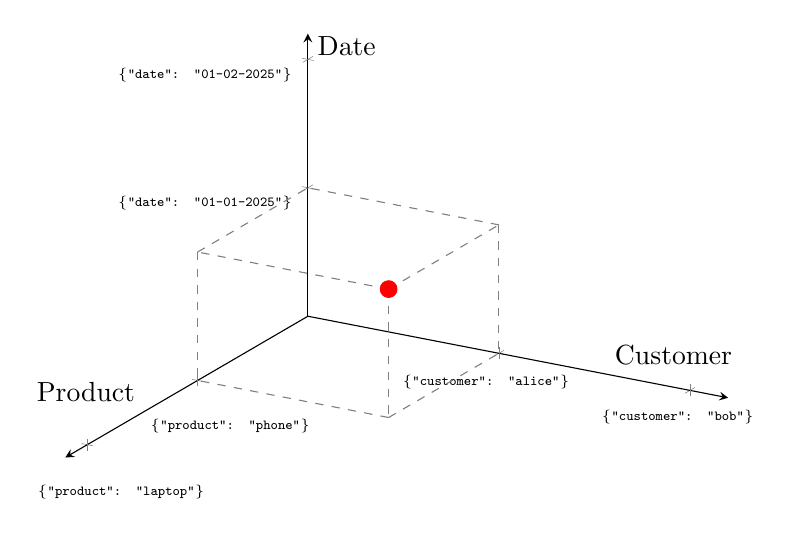
\begin{tikzpicture}
\begin{axis}[
    view={120}{30},
    width=10cm,
    height=8cm,
    grid=major,
    xlabel={Product},
    ylabel={Customer},
    zlabel={Date},
    xtick={1,2},
    ytick={1,2},
    ztick={1,2},
    xticklabels={{\tiny\ttfamily\{"product": "phone"\}}, {\tiny\ttfamily\{"product": "laptop"\}}},
    yticklabels={{\tiny\ttfamily\{"customer": "alice"\}}, {\tiny\ttfamily\{"customer": "bob"\}}},
    zticklabels={{\tiny\ttfamily\{"date": "01-01-2025"\}}, {\tiny\ttfamily\{"date": "01-02-2025"\}}},
    tick label style={font=\small},
    xmin=0, xmax=2.2,
    ymin=0, ymax=2.2,
    zmin=0, zmax=2.2,
    axis lines=middle
]

% Highlighted red point: (Phone, Alice, 01-01-2025)
\addplot3[
    only marks,
    mark size=3pt,
    color=red
]
coordinates {(1,1,1)};

% Dotted projection lines
\addplot3[dashed, color=gray] coordinates {(1,1,1) (0,1,1)};
\addplot3[dashed, color=gray] coordinates {(1,1,1) (1,0,1)};
\addplot3[dashed, color=gray] coordinates {(1,1,1) (1,1,0)};

% Optional projections
\addplot3[dashed, color=gray] coordinates {(1,1,0) (1,0,0)};
\addplot3[dashed, color=gray] coordinates {(1,1,0) (0,1,0)};
\addplot3[dashed, color=gray] coordinates {(1,0,1) (0,0,1)};
\addplot3[dashed, color=gray] coordinates {(1,0,1) (1,0,0)};
\addplot3[dashed, color=gray] coordinates {(0,1,1) (0,0,1)};
\addplot3[dashed, color=gray] coordinates {(0,1,1) (0,1,0)};

\end{axis}
\end{tikzpicture}
\caption{A 3D visualization of an Order entity defined by three dimensions: Product, Customer, and Date.}
\label{fig:entity3d}
\end{figure}

\noindent The entity represented by the red dot has the following intuitive, flattened representation:
\begin{verbatim}
{
  "product": "phone",
  "customer": "alice",
  "date": "01-01-2025"
}
\end{verbatim}
This flattened structure is the result of a formal decomposition process that we will define in Section 2.3. Formally, the entity is a recursive structure where each dimensional value is itself an entity:
\begin{verbatim}
{
  "product": { "product": "phone" },
  "customer": { "customer": "alice" },
  "date": { "date": "01-01-2025" }
}
\end{verbatim}

\subsection{Primitive Values}

Primitive values are the atomic units of information within an entity. They represent the raw, real-world measurements that give meaning to structured data. Regardless of how complex an entity may appear, its informational content ultimately reduces to a collection of primitive values.

In the recursive structure of entities, primitive values serve as the terminal elements—values that cannot be further decomposed.

\paragraph{Supported Primitive Types:}

\begin{itemize}
  \item \textbf{Text} – arbitrary strings (e.g., names, identifiers)
  \item \textbf{Number} – mathematical numbers
  \item \textbf{Boolean} – logical truth values: \texttt{true}, \texttt{false}
  \item \textbf{Bytes} – raw binary data
  \item \textbf{Date} – calendar dates
  \item \textbf{DateWithTimezone} – calendar date with time zone information
  \item \textbf{Time} – clock times
  \item \textbf{TimeWithTimezone} – time with associated time zone
  \item \textbf{Datetime} – combination of date and time without timezone
  \item \textbf{Timestamp} – a specific point in time, typically with high resolution
\end{itemize}

\bigskip
\noindent These primitive types are chosen to cover the full spectrum of values encountered in real-world data, from temporal measurements to textual identifiers and binary blobs.

\subsection{Singular Entity and Its Decomposition}

Since the definition of an entity is recursive—each dimension value is itself an entity—we need a well-defined base case to logically complete this recursion. This base case is the \textit{singular entity}.

A singular entity contains exactly one dimension and one primitive value. Formally:

\begin{equation} \label{eq:singular_entity}
e = \{k: v\} \quad \text{where } k \in \text{Dimension Names},\ v \in \text{Primitive Values}
\end{equation}

Because a singular entity contains exactly one dimension and one value, there is no ambiguity about what the value represents. The dimension name serves only as a label, not as structural information. Therefore, we can reduce the entity to its primitive value alone—relying on the surrounding context to identify the dimension if needed. Owing to this observation, we can define a decomposition function \( \delta \) that strips the structure down to the primitive value:

\begin{equation} \label{eq:decomposition}
\delta : E_{\text{singular}} \to V, \quad \delta(\{k: v\}) = v
\end{equation}

\( E_{\text{singular}} \) is the set of all singular entities, and \( V \) is the set of all primitive values.

Its inverse reconstructs the singular entity from the primitive:

\begin{equation} \label{eq:reconstruction}
\delta^{-1}_k(v) = \{k: v\}
\end{equation}

\noindent Example:
\begin{align} \label{eq:example_decomposition}
\delta(\texttt{\{"product": "phone"\}}) &= \texttt{"phone"}
\end{align}
\begin{align} \label{eq:example_reconstruction}
\delta^{-1}_{\texttt{product}}(\texttt{"phone"}) &= \texttt{\{"product": "phone"\}}
\end{align}

Using \( \delta \) (Eq.~\ref{eq:decomposition}), we can simplify the recursive entity shown after Figure~\ref{fig:entity3d} into the flattened dictionary of primitives shown first.

\subsection{Entity Retrieval Function \texorpdfstring{\( \mu \)}{μ}}

Real-world data sources rarely expose all entities in bulk. Instead, they typically expose \textit{queryable interfaces} that return a \textit{subset} of entities based on partial dimension constraints. To formalize this, we define a retrieval function that maps queries to entity subsets.

Let:
\begin{itemize}
  \item \( E = D_1 \times D_2 \times \dots \times D_n \) be the full theoretical space of entities, as defined in Eq.~\ref{eq:entity_definition}.
  \item \( Q \) be the query domain, defined as the set of all partial entities (dictionaries) formed from a subset of dimensions \( \{D_{i_1}, \dots, D_{i_k}\} \subseteq \{D_1, \dots, D_n\} \). A query \( q \in Q \) is a dictionary of the form \( q = \{d_{i_1}: v_{i_1}, \dots, d_{i_k}: v_{i_k}\} \).
\end{itemize}

The dimensions \( \{D_{i_j}\} \) are those for which the full set of values can be enumerated by systems external to the source system. This enumeration may be achieved through various means, such as referencing a static list of entities, using a separate entity retrieval function, or automatically iterating over values—for example, enumerating dates one by one.

We define the retrieval function:
\begin{equation} \label{eq:retrieval_function}
\mu : Q \rightarrow \mathcal{P}(E)
\end{equation}

Here \( \mathcal{P}(E) \) refers to the power set of \( E \)—the set of all subsets of \( E \). A query \(q\) returns the set of all entities in \(E\) that contain the query as a subset:

\begin{equation} \label{eq:retrieval_query}
\mu(q) = \left\{ e \in E \;\middle|\; q \subseteq e \right\}
\end{equation}

\noindent In this context, \( q \subseteq e \) means that all key-value pairs in the query map \(q\) are also present in the entity map \(e\). This formulation directly models the semantics of filtering operations where multiple constraints must be met.

\bigskip
\noindent\textbf{Special Case – Full Match:}
If \( q \) specifies all \( n \) dimensions (i.e., is a full entity), then:
\begin{equation} \label{eq:full_match}
\mu(q) =
\begin{cases}
\{q\} & \text{if } q \in E \\
\emptyset & \text{otherwise}
\end{cases}
\end{equation}

This becomes a set membership check:
\begin{equation} \label{eq:set_membership}
f_{\text{exists}}(e) = 
\begin{cases}
\text{true} & \text{if } e \in \mu(e) \\
\text{false} & \text{otherwise}
\end{cases}
\end{equation}

\bigskip
\noindent
\textbf{Examples of \( \mu \):}
\begin{itemize}
  \item REST API query: \texttt{GET /orders?customer=alice\&date=2025-01-01}
  \item SQL: \texttt{SELECT * FROM orders WHERE customer = 'alice' AND date = '2025-01-01'}
  \item GraphQL/report filters
\end{itemize}

\noindent The function \( \mu \) defined in Eq.~\ref{eq:retrieval_function} and Eq.~\ref{eq:retrieval_query} captures the query semantics of the source and forms the core interface through which Connector Studio extracts data.

\subsection{Extraction Process}

As defined in Equation~\ref{eq:entity_definition}, the theoretical entity space \( E = D_1 \times D_2 \times \dots \times D_n \) represents all possible entities based on the Cartesian product of dimension sets. However, real-world source systems typically contain only a limited subset of these entities.

We denote this subset as \( E_{\text{actual}} \subseteq E \), which includes all entities that are actually present in the source system and can be discovered via queries supported by the source interface.

To extract data from the source system, Connector Studio enumerates all possible queries from the query domain \( Q = D_{i_1} \times D_{i_2} \times \dots \times D_{i_k} \), where the dimensions \( D_{i_j} \) are those for which values can be externally enumerated (e.g., known customer IDs or dates).

For each query \( q \in Q \), the retrieval function \( \mu \) (as defined in Equation~\ref{eq:retrieval_function}) returns a subset of matching entities:
\[
\mu(q) \subseteq E
\]

By evaluating \( \mu \) over all possible queries in \( Q \), we can recover the total extractable entity set:

\begin{equation} \label{eq:extraction_process}
E_{\text{actual}} = \bigcup_{q \in Q} \mu(q)
\end{equation}

This formulation ensures that Connector Studio’s data extraction process is both complete and computable, as long as:
\begin{itemize}
  \item The values in \( Q \) can be fully enumerated.
  \item The source system provides function \( \mu \).
\end{itemize}

\paragraph{Key Observations:}
\begin{itemize}
  \item \( E_{\text{actual}} \) is discoverable through a finite set of queries as long as \( Q \) is finite.
  \item If \( Q = E \), the extraction becomes exhaustive and equivalent to iterating over the entire theoretical space—though this is rarely feasible in practice.
\end{itemize}

The extraction process is the operational realization of the retrieval function \( \mu \) across the finite, enumerable domain \( Q \), yielding the set \( E_{\text{actual}} \) of discoverable entities.

\subsection{Enumerability of Temporal Dimensions}

The computability of the extraction process described in Equation~\ref{eq:extraction_process} relies on the query domain \( Q \) being finite. However, certain dimensions used in the query domain \( Q \)—most notably, \textit{date-related dimensions}—are technically infinite. For example, the dimension \( D_{\text{date}} \) may span all possible calendar dates, including those far into the future and the past. Despite this, such dimensions are still valid candidates for inclusion in \( Q \) because they are \textit{practically enumerable} at any point in time.

Connector Studio exploits the fact that real-world data extraction typically requires access to a finite history of data, rather than the entire historical timeline. To address this, Connector Studio introduces the concept of a \textbf{historical date}, which is a predefined point in the past (e.g., 5 years ago) from which the enumeration of dates begins during the initial sync. This ensures that the extraction process does not attempt to enumerate dates infinitely far back in time, focusing instead on a relevant historical window. Also, future dates are not included as they do not yield any data.

Thus, while the full theoretical set of dates may exist in \( D_{\text{date}} \), the practically enumerable subset at any given time is:

\begin{equation} \label{eq:practical_dates}
D_{\text{date}}^{\text{practical}}(t) \subseteq D_{\text{date}}
\end{equation}

\paragraph{Pause-Resume Semantics:}

Connector Studio handles the unbounded nature of temporal dimensions via a \textbf{pause-resume mechanism}. This allows continuous yet incremental extraction:

\begin{itemize}
  \item At time \( t \), the extraction process enumerates values in \( D_{\text{date}}^{\text{practical}}(t) \), covering only dates from the historical point to the current date during the initial sync.
  \item Once the extraction reaches the present date, the process is \textit{ended}.
  \item The current date \( t \) is stored persistently in the source log state.
  \item In the next run, extraction resumes from the stored timestamp and continues until the then-current date.
\end{itemize}

Hence, at any point \( t \), after the initial sync, \( D_{\text{date}}^{\text{practical}}(t) \) is a set of dates from the date stored in the checkpoint to the current date:

\begin{equation} \label{eq:practical_dates_checkpoint}
D_{\text{date}}^{\text{practical}}(t) = \{ \text{dates from the checkpoint date up to current date } t \}
\end{equation}

The extraction process in the presence of temporal dimensions (which are infinite) is never truly complete; it is paused and resumed as time progresses.

\section{Saras ETL Platform Basics}

In Saras's ETL platform, an entity set such as "Orders" or "Customers" is referred to as a \textbf{Table}. While Connector Studio is responsible for defining the logic to extract entities from a source system, the ETL platform provides a suite of foundational services that orchestrate and operationalize this extraction logic.

The key services provided by the ETL platform are described below:

\subsection{Job Scheduling}

The platform automatically schedules and executes extraction processes at user-defined frequencies. Each scheduled execution is called a \textbf{sync}.

\subsection{State Checkpointing}

After every successful sync, the ETL platform records the state of the extraction process—such as the most recent date or cursor processed. This \textbf{checkpointed state} ensures that subsequent syncs resume from the exact point where the last successful one ended. The state is stored in a PostgreSQL table called "source\_log"; hence, the checkpointed state is also referred to as the "source log state".

\subsection{Gcs Cache File Storage}

Connector Studio can optionally persist extracted entities into intermediate cache files. These cache files are stored in google cloud storage.

\subsection{Data Type Transformation}

Source systems often use data types that differ from those used in analytical warehouses. The ETL platform automatically performs \textbf{type transformations} to convert source-native types into formats optimized for the target warehouse.

\subsection{Data Loading into Warehouses}

Once data is extracted and transformed, the ETL platform handles the process of \textbf{loading data into warehouses} such as BigQuery, Snowflake, Redshift, etc.

\section{Connector Studio Components}

Connector Studio is designed as a no-code tool that allows users to define data extraction logic seamlessly using modular building blocks. The main components in Connector Studio include \textbf{Entity Sources}, which define how data is retrieved from source systems, and \textbf{Dimension Enumerators}, which help enumerate entities for a particular dimension in order to construct the query domain \( Q \) (see section 2.5) for extracting data.

\subsection{Entity Sources}

An \textbf{Entity Source} is the foundational component in Connector Studio that encapsulates all the logic required to extract entities from a specific entity set in a source system. Each Entity Source is designed to interact with a particular type of data source (e.g., databases, APIs, files). The Entity Sources vary in terms of the methods they use to extract data, but they all perform one primary task—retrieve entities from the source system.

There are multiple types of Entity Sources in Connector Studio, categorized based on the nature of the entity retrieval function \( \mu \) (see section 2.4) given by the source system. Below is an organized explanation of these components:

\subsubsection{General Entity Sources}
These Entity Sources interact with APIs and reports to extract data:
\begin{itemize}
    \item \textbf{APIEntitySource:} Retrieves entities by making structured requests to APIs (e.g., REST, SOAP). It typically supports customizable filter parameters, such as querying specific orders based on customer or date.
    \item \textbf{ReportEntitySource:} Extracts data from pre-generated reports in formats like CSV, Excel, or JSON.
\end{itemize}

\subsubsection{Database Entity Sources}
Database Entity Sources connect directly to relational databases and allow data extraction through SQL queries. The specific types of database sources supported include:
\begin{itemize}
    \item \textbf{PostgresDatabaseEntitySource:} Designed for interacting with PostgreSQL databases.
    \item \textbf{MySQLDatabaseEntitySource:} Designed for interacting with MySQL databases.
\end{itemize}

\subsubsection{File Entity Sources}
File Entity Sources extract entities from files stored in cloud-based storage systems.
\begin{itemize}
    \item \textbf{AmazonS3FileEntitySource:} For extracting entities from files stored in Amazon S3.
    \item \textbf{GoogleCloudStorageFileEntitySource:} For files stored in Google Cloud Storage.
    \item \textbf{SFTPFileEntitySource:} For securely retrieving files from SFTP servers.
\end{itemize}

\subsubsection{Ordered Entity Sources}
Ordered Entity Sources are a special category of Entity Sources that produce entities that have an intrinsic order defined by some comparator function, typically representing temporal data, such as dates or timestamps. These sources are essential for defining ranges in queries, such as extracting all orders within a date range. Examples include:
\begin{itemize}
    \item \textbf{DateEntitySource:} Produces sequential dates.
    \item \textbf{DatetimeEntitySource:} Produces sequential datetime values.
    \item \textbf{TimestampEntitySource:} Generates sequential timestamps.
    \item \textbf{WeekEntitySource:} Produces weeks sequentially
\end{itemize}

Ordered Entity Sources support retrieving the next or previous entity relative to a given one, and they allow specifying a step (difference/skip) when moving forward or backward. They also expose the minimum and maximum entities supported by them. These capabilities are critical when working with Entity Sources that require finite input ranges, such as a start and end date.

\subsection{Dimension Enumerators}

The \textbf{Dimension Enumerator} is another core component of Connector Studio. It is responsible for enumerating entities belonging to a particular dimension in the query domain \( Q \). Because a dimension is itself an entity set, an entity source is used to enumerate it. Thus, a dimension enumerator requires an entity source attached to it which is used to enumerate entities of that dimension. 

Multiple dimension enumerators can be attached to an entity source, one for each dimension in the query domain \( Q \). At runtime, a cartesian product of the entities enumerated by all dimension enumerators is calculated and used by the entity source to pass into the entity retrieval function \( \mu \).

Entity Sources and Dimension Enumerators together form a hierarchical tree structure to define and execute the data extraction process.

\subsubsection{Types of Dimension Enumerators:}
There are two key types of Dimension Enumerators in Connector Studio:

\begin{itemize}
    \item \textbf{Parent Dimension Enumerator:} A simple enumerator that passes through the entities generated by its attached Entity Source without modification.

    \item \textbf{Range Dimension Enumerator:} A specialized enumerator designed to work with ordered entity sources. It consumes a sequence of ordered entities (e.g., dates) and transforms it into a sequence of range entities. For instance, it might take dates from a DateEntitySource and produce monthly ranges, where each range is an entity with "lowerBound" and "upperBound" dimensions. This is essential for querying APIs that require a start and end date.
\end{itemize}

\section{Entity Source Template}

The core components—Entity Sources and Dimension Enumerators—are practically configured by a connector builder using a JSON structure known as the \textbf{Entity Source Template}. This template serves as the complete blueprint for extracting a single entity set (e.g., "Orders," "Events") from a source system. It declaratively defines the tree of components, the data retrieval logic, and the state management required for data extraction.

Each extraction process for an entity set is defined by one such template. Below, we dissect the structure of a typical template, followed by a complete example.

\subsection{Key Components of the Template}

An Entity Source Template is a JSON object with several key top-level properties:

\begin{itemize}
    \item \textbf{"initialAuthenticationContext":} The authencitcation context variables for the first sync of the table.
    
    \item \textbf{"contextVariables":} Generic context variables which are available to a running extraction process for variable injection.

    \item \textbf{"shouldSendDataToWarehouse":} A boolean (`"true"`/`"false"`) indicating if the extracted entities should be loaded into the destination warehouse. This can be set to \texttt{"false"} if the table's only purpose is to populate the gcs cache for other, dependent "child" tables.

    \item \textbf{"enableGcsCaching":} A boolean flag. When set to \texttt{"true"}, Connector Studio persists the entities emitted by this template into a cache file in Google Cloud Storage. Each cache file is tagged with the \textit{Logical Sync Sequence Number} and the \textit{Hibernation Sequence Number} of the sync that produced it (see Sync Hibernation section). Dependent templates can read these files via GcsCacheEntitySource; access can be scoped by the \texttt{"gcsCachingChildTableCohort"}. When set to \texttt{"false"}, no cache files are written.

    \item \textbf{"gcsCachingChildTableCohort":} A string identifier used to group dependent tables. The GcsCacheEntitySource(see section 19) with the same "cohort" in other entity source templates can access the cache file created by this template.

    \item \textbf{"gcsCacheEntityTransformationOps":} A list of json ops(see section 16.1) which will be applied on the entities extracted before storing them in entity cache. This is mostly useful to save storage space by omitting fields in the entities which are not useful for dependent extraction processes.

    \item \textbf{"appendPreviousLogicalSyncEntitiesInGcsCache":} A boolean flag. If \texttt{"true"}, entities from the previous logical sync(see Sync Hibernation section) are carried over into the new cache file, creating a cumulative cache over time.

    \item \textbf{"entitySourceType":} The type of the root level entity source.
    
    \item \textbf{"params":} Params of the root level entity source.

    \item \textbf{"initialSyncSourceLogState":} The source log state of an implicit 0th sync. The first sync uses this state as its starting point.

    \item \textbf{"entityProcessorParams":} Params of the entity processor.
\end{itemize}

Note: A "Table" is a terminology in saras's ETL platform. It means the extraction process for a particular entity set in a source.

\subsection{Example Template}
The following example illustrates a complete Entity Source Template for retrieving "return-registrations" from a sample API endpoint. This template demonstrates how the components work together to handle parameterized API requests, date-based range queries, cursor-based pagination, and complex response parsing.

\vspace{3em}

\begin{lstlisting}[language=json]
{
  "initialAuthenticationContext": {
    "parcellab_ac": {
      "basic_token": "b64(<<services_accountid>>:<<services_api_token>>)"
    }
  },
  "contextVariables": {},
  "shouldSendDataToWarehouse": "true",
  "enableGcsCaching": "false",
  "gcsCachingChildTableCohort": "",
  "gcsCacheEntityTransformationOps": [],
  "appendPreviousLogicalSyncEntitiesInGcsCache": "false",
  "entitySourceType": "API_ENTITY_SOURCE",
  "params": {
    "memoryEfficientDimensionName": "datetime",
    "entityFieldTypeCastTemplate": {},
    "postExtractionEntityFilter": {},
    "postExtractionEntityNegativeFilter": {},
    "firstPaginatedCallApiInput": {
      "requestBodyType": "NONE",
      "requestBody": {},
      "queryParams": {
        "updated_at_after": "{{$.datetime.lowerBound.datetime}}",
        "updated_at_before": "{{$.datetime.upperBound.datetime}}"
      },
      "headerParams": {
        "Authorization": "Parcellab-API-Token {{$.basic_token}}",
        "Accept": "application/json"
      }
    },
    "remainingPaginatedCallsApiInput": {
      "requestBodyType": "NONE",
      "requestBody": {},
      "queryParams": {
        "cursor": "{{$.cursor}}",
        "updated_at_after": "{{$.datetime.lowerBound.datetime}}",
        "updated_at_before": "{{$.datetime.upperBound.datetime}}"
      },
      "headerParams": {
        "Authorization": "Parcellab-API-Token {{$.basic_token}}",
        "Accept": "application/json"
      }
    },
    "entitySourceName": "Returns_Registrations",
    "requestMethod": "GET",
    "endpoint": "https://api.parcellab.com/v4/returns/return-registrations/",
    "remainingPaginatedCallsSameAsFirstCall": false,
    "actionScript": "aWYgKGN1cnJlbnRTeW5jU3RhdHMuZ2V0TWlsbGlTZWNvbmRzRWxhcHNlZEZyb21TeW5jU3RhcnQoKSA+IDE4MDAwMDApIHsgbmV3IEhpYmVybmF0ZUFuZFJldHJ5KDAsIG5ldyBMb2dnaW5nQ29uZmlndXJhdGlvbihmYWxzZSwgZmFsc2UpKTsgfSBlbHNlIGlmIChhcGlPdXRwdXQucmVzcG9uc2VDb2RlID09IDIwMCkgeyBuZXcgU2xlZXBBbmROZXh0UGFnZUNhbGwoMCwgbmV3IExvZ2dpbmdDb25maWd1cmF0aW9uKHRydWUsIGZhbHNlKSk7IH0gZWxzZSBpZiAoYXBpT3V0cHV0LnJlc3BvbnNlQ29kZSA9PSA0MjkgJiYgYXBpT3V0cHV0LnJlc3BvbnNlSGVhZGVyc1sicmV0cnktYWZ0ZXIiXSkgeyBuZXcgU2xlZXBBbmRSZXRyeShOdW1iZXIoYXBpT3V0cHV0LnJlc3BvbnNlSGVhZGVyc1sicmV0cnktYWZ0ZXIiXSkgKiAxMDAwLCBuZXcgTG9nZ2luZ0NvbmZpZ3VyYXRpb24odHJ1ZSwgdHJ1ZSkpOyB9IGVsc2UgeyBuZXcgVGhyb3dFeGNlcHRpb24oIkZhaWxlZCB3aXRoIHN0YXR1cyBjb2RlOiAiICsgYXBpT3V0cHV0LnJlc3BvbnNlQ29kZSwgbmV3IExvZ2dpbmdDb25maWd1cmF0aW9uKHRydWUsIHRydWUpKTsgfQ==",
    "extraFieldsToAddInEntity": {},
    "dimensionEnumerators": [
      {
        "dimensionEnumeratorType": "RANGE_DIMENSION_ENUMERATOR",
        "params": {
          "dimensionName": "datetime",
          "initialSyncLowerBoundEntity": {
            "datetime": "<<$.start_date_datetime_hist_strategy>>"
          },
          "rangePartitionStrategyMetadata": {
            "partitionSize": "86400000",
            "skipValueForEntityToSaveInSourceLog": "-<<$.lookbackValues.lookbackInMillis>>",
            "skipValueForMinEntityOfNextPartition": "0"
          },
          "rangePartitionStrategyType": "FIXED_PARTITION_SIZE_PARTITION_STRATEGY",
          "dimensionSource": {
            "entitySourceType": "DATETIME_ENTITY_SOURCE",
            "params": {
              "datetimePattern": "yyyy-MM-dd'T'HH:mm:ss'Z'",
              "zoneId": "UTC",
              "timeLag": "0",
              "entitySourceName": "datetime"
            }
          }
        }
      }
    ],
    "paginationType": "CURSOR_BASED",
    "initialPaginationControllerParams": {
      "initialPageNumber": "1"
    },
    "authenticationType": "STATIC",
    "authenticationControllerParams": {
      "id": "parcellab_auth",
      "authenticationContextId": "parcellab_ac"
    },
    "entityExtractionChain": [
      {
        "operationName": "select",
        "params": {
          "fieldsToInclude": [
            "results"
          ]
        }
      },
      {
        "operationName": "decomposeArrayField",
        "params": {
          "fieldToDecompose": "results"
        }
      },
      {
        "operationName": "flatten",
        "params": {
          "fieldToFlatten": "results"
        }
      },
      {
        "operationName": "stringifyField",
        "params": {
          "fieldToStringify": "additional_fields"
        }
      }
    ],
    "paginationMetadataChain": [
      {
        "operationName": "select",
        "params": {
          "fieldsToInclude": [
            "responseBody"
          ]
        }
      },
      {
        "operationName": "flatten",
        "params": {
          "fieldToFlatten": "responseBody"
        }
      },
      {
        "operationName": "select",
        "params": {
          "fieldsToInclude": [
            "next"
          ]
        }
      },
      {
        "operationName": "decomposeUrl",
        "params": {
          "urlFieldToDecompose": "next"
        }
      },
      {
        "operationName": "applyJsonPathOnField",
        "params": {
          "fieldToApplyJsonPathOn": "next",
          "jsonPath": "$.queryParams"
        }
      },
      {
        "operationName": "flatten",
        "params": {
          "fieldToFlatten": "next"
        }
      },
      {
        "operationName": "select",
        "params": {
          "fieldsToInclude": [
            "cursor"
          ]
        }
      },
      {
        "operationName": "removeUrlEncoding",
        "params": {
          "urlFieldToRemoveEncoding": "cursor"
        }
      }
    ]
  },
  "initialSyncSourceLogState": {
    "entitySourceType": "API_ENTITY_SOURCE",
    "dimensionEnumeratorsState": {
      "datetime": {
        "dimensionName": "DATETIME",
        "dimensionEnumeratorType": "RANGE_DIMENSION_ENUMERATOR",
        "backingEntitySourceState": {},
        "lowerBoundEntity": {
          "datetime": "<<$.start_date_datetime_hist_strategy>>"
        }
      }
    }
  },
  "entityProcessorParams": {
    "autoDetectNewColumns": "true",
    "detectDataTypeChanges": "true",
    "stringParsingConfiguration": {
      "entityLevelParsingOrder": [
        "TIMESTAMP",
        "DATETIME",
        "TIME",
        "DATE",
        "STRING"
      ],
      "fieldSpecificParsingOrder": {}
    },
    "additionalDatePatterns": [],
    "additionalDateTimePatterns": [],
    "additionalTimePatterns": [],
    "additionalTimeStampPatterns": [],
    "dataTypeChangeRestrictions": [],
    "enableHackyColumnNameStandardization": "false"
  }
}
\end{lstlisting}

\section{Context Variable Pool}

During the extraction process, Connector Studio maintains a dynamic in-memory key-value store called the \textbf{Context Variable Pool}. This pool acts like a shared working memory, providing a centralized location for storing, reading, and updating variables throughout the execution lifecycle of the extraction. The variable pool is modeled as a JSON object where keys represent the variable names and values (which can be any valid json value including string, number, json object, json array etc) are the values of the variables.

\subsection{Purpose and Usage}

The Context Variable Pool enables flexible data injection into different parts of the extraction process. Variables in this pool are typically used to inject values dynamically into API URLs and parameters, or to pass computed or derived values between different stages of extraction.

\subsection{Variable Access Syntax}

As the variable pool is essentially a json, json-path is used to access values in it. Values from the pool are injected into the entity source template using \texttt{\{\{json-path\}\}} syntax.

\subsection{Scope and Mutability}

The pool is available globally to the entire extraction process and behaves like a mutable dictionary:
\begin{itemize}
  \item \textbf{Read:} Variables can be accessed at any injection point using the syntax shown above.
  \item \textbf{Write:} Variables can be added or updated during intermediate stages of execution (e.g., authentication response processing, cursor extraction, etc.).
  \item \textbf{Delete:} Variables can be removed if no longer needed.
\end{itemize}

\subsection{Example}

Given the following context variable pool:
\begin{verbatim}
{
  "shop_name": {
    "name": "tryearthbreeze"
  },
  "version": "2023-07",
  "access_token": "abc123xyz"
}
\end{verbatim}

You can inject these values into the API configuration:
\begin{verbatim}
"endpoint": "https://{{$.shop_name.name}}.mysource.com/admin/api/{{$.version}}/events.json",
"headerParams": {
  "Access-Token": "{{$.access_token}}"
}
\end{verbatim}

This will evaluate to:
\begin{verbatim}
endpoint: https://tryearthbreeze.mysource.com/admin/api/2023-07/events.json
header: Access-Token: abc123xyz
\end{verbatim}

\section{Function Guided Injection}

The injection syntax using \texttt{\{\{json-path\}\}} supports string substitution from the context variable pool. However, in many real-world cases, you may need to inject types other than strings—such as numbers, arrays, or JSON objects at the injection point. Additionally, you might want to transform the values retrieved from the pool before injecting them (e.g., base64 encoding, trimming whitespace, typecasting, etc.).

\textbf{Function Guided Injection} extends the basic injection mechanism by allowing functions to be applied to the values retrieved from the context variable pool before they are injected. The general syntax is:

\begin{verbatim}
{{function_name(json-path)}}
\end{verbatim}

This tells Connector Studio to first retrieve the value at the specified JSON path from the context variable pool, apply the function \texttt{function\_name} to it, and then inject the result at the target location in the entity source template.

\textbf{Important:} Each function guided injection can only be used when the entire value at the injection point must be the type produced by the function. You cannot mix it with surrounding strings. For example:
  \begin{verbatim}
  "sample": "{{inject_json($.varA)}}"     is valid
  "sample": "abc xyz {{inject_json($.varA)}}"  is invalid
  \end{verbatim}

\subsection{Supported Functions}

\begin{itemize}
  \item \textbf{\texttt{typecast\_number}}:  
  Attempts to convert the referenced value into a JSON number. The conversion behavior is as follows:
  \begin{itemize}
    \item If the value is already a number, it is injected as-is.
    \item If it is a string representing a valid number (e.g., \texttt{"42.5"}), it is converted and injected as a number.
    \item If the value is a boolean, JSON array, object, null, or a non-numeric string, an exception is thrown.
  \end{itemize}

  \textbf{Example:}
  \begin{itemize}
    \item Context Variable Pool:
    \begin{verbatim}
    {
      "varA": "123.33"
    }
    \end{verbatim}

    \item Entity Source Template Snippet:
    \begin{verbatim}
    {
      "amount": "{{typecast_number($.varA)}}"
    }
    \end{verbatim}

    \item Result after Injection:
    \begin{verbatim}
    {
      "amount": 123.33
    }
    \end{verbatim}
  \end{itemize}

  \item \textbf{\texttt{typecast\_boolean}}: Converts the referenced value into a JSON boolean. 
  \begin{itemize}
    \item If the value is already a boolean, it is injected as-is.
    \item If it is a string, the string is converted to lowercase and should be either \texttt{"true"} or \texttt{"false"} after conversion.
    \item For all other types, an exception is thrown.
  \end{itemize}
  
  \textbf{Example:}
  \begin{itemize}
    \item Context Variable Pool:
    \begin{verbatim}
    {
      "varA": "True"
    }
    \end{verbatim}

    \item Entity Source Template Snippet:
    \begin{verbatim}
    {
      "isActive": "{{typecast_boolean($.varA)}}"
    }
    \end{verbatim}

    \item Result after Injection:
    \begin{verbatim}
    {
      "isActive": true
    }
    \end{verbatim}
  \end{itemize}

  \item \textbf{\texttt{inject\_json}}: Injects any arbitrary JSON (can be a JSON object, JSON array, number, boolean, string, or null) into the injection point.

  \textbf{Example:}
  \begin{itemize}
    \item Context Variable Pool:
    \begin{verbatim}
    {
      "varA": {
        "key1": [
            1,
            2,
            3
        ]
      }
    }
    \end{verbatim}

    \item Entity Source Template Snippet:
    \begin{verbatim}
    {
      "abc": "{{inject_json($.varA)}}"
    }
    \end{verbatim}

    \item Result after Injection:
    \begin{verbatim}
    {
      "abc": {
        "key1": [
            1,
            2,
            3
        ]
      }
    }
    \end{verbatim}
  \end{itemize}

  \item \textbf{\texttt{inject\_json\_array\_join\_with\_comma}}: Joins all the primitive values (string, boolean, number) of the JSON array pointed to by the given JSON path in the context variable pool into a string using the separator ',' and injects it at the injection point.

  \textbf{Example:}
  \begin{itemize}
    \item Context Variable Pool:
    \begin{verbatim}
    {
      "varA": {
        "key1": [
            1,
            2,
            3
        ]
      }
    }
    \end{verbatim}

    \item Entity Source Template Snippet:
    \begin{verbatim}
    {
      "abc": "{{inject_json_array_join_with_comma($.varA.key1)}}"
    }
    \end{verbatim}

    \item Result after Injection:
    \begin{verbatim}
    {
      "abc": "1,2,3"
    }
    \end{verbatim}
  \end{itemize}

  \item \textbf{\texttt{base64}}: Base64 encodes the referenced value and injects it at the injection point. The referenced value has to be a string.

  \textbf{Example:}
  \begin{itemize}
    \item Context Variable Pool:
    \begin{verbatim}
    {
      "varA": "abc"
    }
    \end{verbatim}

    \item Entity Source Template Snippet:
    \begin{verbatim}
    {
      "abc": "{{base64($.varA)}}"
    }
    \end{verbatim}

    \item Result after Injection:
    \begin{verbatim}
    {
      "abc": "YWJj"
    }
    \end{verbatim}
  \end{itemize}

\end{itemize}

\section{Sync Hibernation}

The extraction process in Connector Studio is designed to run until all entities in the query domain \( Q \) (see Equation~\ref{eq:extraction_process}) have been enumerated. However, this comprehensive process can lead to significant latency, as it may take several hours or even days to complete. To mitigate this, Connector Studio features a mechanism called \textbf{Sync Hibernation}.

Sync Hibernation ensures that any given extraction process (also termed as  \textbf{logical sync}) is divided into multiple shorter sessions, known as \textbf{hibernated syncs}. Each hibernated sync runs for a predefined duration, such as 30 minutes (configurable), after which the in-memory state of the sync is captured and stored as a checkpoint. When the next hibernated sync begins, this state is restored, allowing the process to resume precisely from where it left off in the previous session. This approach ensures that data is delivered to the warehouse incrementally, reducing latency and improving data freshness.

Each sync or job in Saras's ETL platform is assigned two identifiers:

- \textbf{Logical Sync Sequence Number:} This identifier (starting from 1) represents the sequence of the overall logical sync, providing an identifier for the complete extraction process.
  
- \textbf{Hibernation Sequence Number:} This identifier (starting from 1) indicates the sequence of a specific hibernated sync within a logical sync.

\section{Post Extraction Entity Filter}

The Post Extraction Entity Filter provides a declarative way to retain only entities that satisfy a set of field equality conditions after they have been extracted, but before they are emitted by an Entity Source. Conceptually, it acts as an inclusion predicate: if the entity satisfies every condition specified in the filter, it is forwarded; otherwise, it is dropped.

\subsection{Scope and Placement}

\begin{itemize}
  \item The filter is configured per Entity Source in its params under the field \texttt{"postExtractionEntityFilter"}.
  \item It applies to all Entity Sources except Ordered Entity Sources (e.g., DateEntitySource, DatetimeEntitySource, TimestampEntitySource, WeekEntitySource).
\end{itemize}

\subsection{Schema}

The filter is a JSON object whose keys are field names within the extracted entity. The shape of the filter mirrors the shape of the entity being matched, and each value can be one of:

\begin{itemize}
  \item \textbf{Primitive value} (text, number, boolean, etc.): A direct equality target for that field in the entity (for example, \texttt{"status": "ACTIVE"}).
  \item \textbf{Nested JSON object:} A sub-filter recursively applied to the corresponding nested object field in the entity.
  \item \textbf{JSON array:} A single-element array containing one sub-filter object. That sub-filter is recursively applied to \emph{every} element of the corresponding array-of-objects field (i.e., a REPEATED RECORD type) in the entity. All elements must satisfy the sub-filter.
\end{itemize}

Field names are direct keys into the entity (not JSON paths). Nesting into sub-objects or array elements is expressed by nesting in the filter structure itself.

\subsection{Evaluation Semantics}

Given an extracted entity \(e\) and the configured filter \(f\):

\begin{itemize}
  \item All key-value pairs in \(f\) are combined with logical AND. The entity \(e\) passes the filter only if every condition holds.
  \item For each key \(k\) in \(f\) with expected value \(v\): the value \(e[k]\) is read from the entity and compared to \(v\). Two values are considered equal only if both their string representations match \emph{and} their runtime types match. The comparison is strictly typed: the string \texttt{"5"} does not match the number \texttt{5}.
  \item \textbf{Missing or null fields are ignored.} If the field referenced by \(k\) is absent in \(e\) or has a value of \texttt{null}, that condition is skipped and treated as passing. As a result, the filter only excludes entities for which the field is present and not equal to the expected value.
  \item Nested objects and arrays are evaluated recursively using the same rules.
\end{itemize}

\subsection{Example}

Suppose the source emits entities of the form:
\begin{lstlisting}[language=json]
{
  "order_id": "A123",
  "status": "FULFILLED",
  "customer": {
    "country": "US",
    "tier": "GOLD"
  },
  "lineItems": [
    { "type": "PRODUCT", "currency": "USD" },
    { "type": "PRODUCT", "currency": "USD" }
  ]
}
\end{lstlisting}

The following filter retains only fulfilled orders, from US gold-tier customers, whose line items are all in USD:
\begin{lstlisting}[language=json]
{
  "postExtractionEntityFilter": {
    "status": "FULFILLED",
    "customer": {
      "country": "US",
      "tier": "GOLD"
    },
    "lineItems": [
      { "currency": "USD" }
    ]
  }
}
\end{lstlisting}

To disable the filter entirely, set it to an empty JSON object: \texttt{"postExtractionEntityFilter": \{\}}. An empty filter passes every entity.

\section{Post Extraction Entity Negative Filter}

The Post Extraction Entity Negative Filter is the companion to the Post Extraction Entity Filter and provides a declarative way to \emph{drop} entities that match any of a set of field equality conditions. Conceptually, it acts as an exclusion predicate: if the entity matches any condition specified in the negative filter, it is dropped; otherwise, it is forwarded.

\textbf{Important:} The negative filter is not the logical inverse of the positive filter. The positive filter combines its conditions with AND, while the negative filter combines its conditions with OR. The two filters are applied independently and sequentially — an entity must pass the positive filter \emph{and} must not match the negative filter to be emitted.

\subsection{Scope and Placement}

\begin{itemize}
  \item The filter is configured per Entity Source in its params under the field \texttt{"postExtractionEntityNegativeFilter"}.
  \item It applies to all Entity Sources except Ordered Entity Sources (e.g., DateEntitySource, DatetimeEntitySource, TimestampEntitySource, WeekEntitySource).
\end{itemize}

\subsection{Schema}

The negative filter is a flat JSON object whose keys are field names within the extracted entity and whose values are the primitive values to exclude on. Unlike the positive filter, only primitive values (text, number, boolean, etc.) are supported — nested JSON objects and nested arrays are not supported in the negative filter.

\subsection{Evaluation Semantics}

Given an extracted entity \(e\) and the configured negative filter \(g\):

\begin{itemize}
  \item All key-value pairs in \(g\) are combined with logical OR. The entity \(e\) is dropped if any condition matches.
  \item For each key \(k\) in \(g\) with excluded value \(v\): the entity is dropped if \(e[k]\) is present (not null) \emph{and} its string representation equals \(v\) \emph{and} its runtime type equals \(v\)'s type. The comparison is strictly typed, just as in the positive filter.
  \item \textbf{Missing or null fields are ignored.} If the field referenced by \(k\) is absent in \(e\) or has a value of \texttt{null}, that condition cannot match and contributes nothing to the OR.
  \item An empty negative filter (\texttt{\{\}}) excludes no entity.
\end{itemize}

\subsection{Example}

Suppose the source emits entities of the form:
\begin{lstlisting}[language=json]
{
  "order_id": "A123",
  "status": "CANCELLED",
  "test_order": true
}
\end{lstlisting}

The following negative filter drops every entity whose \texttt{status} is \texttt{"CANCELLED"} \emph{or} whose \texttt{test\_order} flag is \texttt{true}:
\begin{lstlisting}[language=json]
{
  "postExtractionEntityNegativeFilter": {
    "status": "CANCELLED",
    "test_order": true
  }
}
\end{lstlisting}

To disable the negative filter entirely, set it to an empty JSON object: \texttt{"postExtractionEntityNegativeFilter": \{\}}.

\subsection{Interaction with the Positive Filter}

For every extracted entity, the Entity Source first evaluates the positive filter and then the negative filter:

\begin{itemize}
  \item The entity must satisfy the positive filter (AND of all conditions).
  \item The entity must not match the negative filter (OR of all conditions).
\end{itemize}

Only entities that satisfy both checks are emitted downstream.

\section{Premature Entity Source Termination Strategy}

Some sources expose a temporal attribute (e.g., createdAt, updatedAt) on each entity but do not allow filtering by that attribute in the retrieval function \( \mu \). If such sources also allow the results of \( \mu \) to be ordered in descending order by that same temporal attribute, Connector Studio can avoid re-reading the entire history on every sync by terminating the logical sync early once already-processed history is reached. This capability is called "Premature Entity Source Termination" and it is configured using "Premature Entity Source Termination Strategy".

\subsection{When to Use}
Use this feature for non-ordered Entity Sources (APIs, reports, databases, files) when all of the following hold:
\begin{itemize}
  \item The source can return entities sorted in descending order by a temporal field present in each entity.
  \item The source does not support filtering in \( \mu \) by that temporal field.
  \item You want each logical sync to process only the new “head” of data since the last logical sync, then stop once the iteration enters already-processed history.
\end{itemize}

\subsection{High-Level Behavior}
\begin{itemize}
  \item First logical sync: The source is read to exhaustion (full history) in descending temporal order. The strategy records the maximum temporal value seen, called the \textit{fieldToUseForTerminationValue} in source log state.
  \item Subsequent logical syncs: Reading again starts from the most recent data (still in descending order). As soon as an entity with a temporal value \emph{strictly less than} \textit{fieldToUseForTerminationValue} is encountered, the logical sync terminates immediately because all remaining entities are older and were already processed in prior logical syncs.
  \item Equality is allowed to pass: Entities whose temporal value is equal to \textit{fieldToUseForTerminationValue} are still processed. This ensures that late-arriving entities with the same timestamp are not missed. Downstream deduplication/upsert should handle duplicates if any.
\end{itemize}

\subsection{Configuration}
Each applicable Entity Source can declare a termination strategy in the "prematureEntitySourceTerminationStrategy" field in params.

\paragraph{Schema}
\begin{lstlisting}[language=json]
{
  "prematureEntitySourceTerminationStrategy": {
    "prematureEntitySourceTerminationStrategyType": "NONE" | "DATETIME" | "TIMESTAMP",
    "params": {
      // parameters (see below)
    }
  }
}
\end{lstlisting}

\paragraph{Types}
\begin{itemize}
  \item \texttt{"NONE"}: Disabled. The Entity Source runs to exhaustion (no early termination). There are no params so the "params" is an empty json object.
  \item \texttt{"DATETIME"}: Use when the termination field is a datetime string. Parameters:
  \begin{itemize}
    \item \texttt{fieldToUseForTerminationJsonPath} — JSON path in each emitted entity that resolves to the datetime value (string).
    \item \texttt{datetimePattern} — Pattern used to parse the value (for example, \texttt{"yyyy-MM-dd'T'HH:mm:ss"}). The value must conform exactly to this pattern.
  \end{itemize}
  \item \texttt{"TIMESTAMP"}: Use when the termination field is a timestamp. Parameters:
  \begin{itemize}
    \item \texttt{fieldToUseForTerminationJsonPath} — JSON path in each emitted entity that resolves to the timestamp value (can also be numeric if it represents a 13 digit or 10 digit timestamp).
    \item \texttt{timestampPattern} — How to interpret the number. Supported values:
    \begin{itemize}
      \item \texttt{normal timestamp pattern} - a normal timestamp pattern with zone (for example, \texttt{"yyyy-MM-dd'T'HH:mm:ss.SSSZ"}).
      \item \texttt{"EPOCH\_MILLIS"} — milliseconds since Unix epoch.
      \item \texttt{"EPOCH\_SECONDS"} — seconds since Unix epoch.
    \end{itemize}
  \end{itemize}
\end{itemize}

\paragraph{Examples}
\begin{lstlisting}[language=json]
{
  "...": "...",
  "prematureEntitySourceTerminationStrategy": {
    "prematureEntitySourceTerminationStrategyType": "DATETIME",
    "params": {
      "fieldToUseForTerminationJsonPath": "$.created_at",
      "datetimePattern": "yyyy-MM-dd'T'HH:mm:ss"
    }
  }
}
\end{lstlisting}

\begin{lstlisting}[language=json]
{
  "...": "...",
  "prematureEntitySourceTerminationStrategy": {
    "prematureEntitySourceTerminationStrategyType": "TIMESTAMP",
    "params": {
      "fieldToUseForTerminationJsonPath": "$.updated_at_epoch",
      "timestampPattern": "EPOCH_MILLIS"
    }
  }
}
\end{lstlisting}

\subsubsection*{Configuration Schema in \texttt{initialSyncSourceLogState}}

The \texttt{prematureEntitySourceTerminationStrategyState} object within the \texttt{initialSyncSourceLogState} is used to bootstrap the termination logic for the very first logical sync.

Since the first logical sync is designed to process the full history of the source to establish an initial high-water mark, no pre-existing termination value is needed. The system identifies that a termination strategy is active from the main \texttt{params} configuration and runs the first sync to completion. After this sync finishes, it populates the source log state with the maximum temporal value it discovered, which will then be used by all subsequent logical syncs.

Therefore, for the initial sync, the state object must be an empty JSON object \texttt{\{\}}.

\paragraph{Schema}
\begin{lstlisting}[language=json]
{
  "...": "...",
  "prematureEntitySourceTerminationStrategyState": {},
  "...": "..."
}
\end{lstlisting}

\paragraph{Note on Subsequent Syncs}
While the initial state is empty, the source log state saved after the first successful logical sync will be populated. For example, it might look like this:
\begin{lstlisting}[language=json]
{
  "fieldToUseForTerminationValue": "2025-07-01T15:30:00"
}
\end{lstlisting}
This \texttt{fieldToUseForTerminationValue} is then read at the start of the next logical sync to enable the early termination behavior.

\section{Date Entity Source}

The Date Entity Source is an ordered entity source that produces a sequence of calendar dates. It is typically used to build date ranges via the Range Dimension Enumerator. The sequence runs from the Unix epoch up to the current date in a specified time zone, offset by a configurable time lag, ensuring a finite, computable set at runtime.

\subsection{When to Use}
Use the Date Entity Source when:
\begin{itemize}
  \item A daily step is the natural unit for enumeration (1 step = 1 day).
  \item An API expects dates (not datetimes or timestamps) as inputs.
\end{itemize}

\subsection{Emitted Entity Shape}
Each emitted entity represents one calendar date and contains:
\begin{itemize}
  \item \texttt{"date"} — Text, formatted using the configured pattern (for example, \texttt{"2025-07-01"}).
  \item \texttt{"day"} — Text representing the day of month (for example, \texttt{"1"} through \texttt{"31"}).
  \item \texttt{"month"} — Text representing the month (for example, \texttt{"1"} through \texttt{"12"}).
  \item \texttt{"year"} — Text representing the year (for example, \texttt{"2025"}).
\end{itemize}

Example:
\begin{lstlisting}[language=json]
{
  "date": "2025-07-01",
  "day": "1",
  "month": "7",
  "year": "2025"
}
\end{lstlisting}

\subsection{Runtime Semantics}
At runtime, the entity source enumerates dates in ascending order with a daily step, over a closed interval [min, max]:
\begin{itemize}
  \item min = the Unix epoch date (1970-01-01).
  \item max = today - \texttt{timeLag}, in the specified time zone.
\end{itemize}
Both \textit{min} and \textit{max} are inclusive. ``Today'' is evaluated in the configured time zone. The entity source also exposes a natural total ordering on dates and supports moving forward or backward by a specified number of days. It also supports getting the max date and min date.

\subsection{Configuration Schema}
Configure the Date Entity Source inside any component that accepts an ordered entity source (for example, a Range Dimension Enumerator).

\begin{lstlisting}[language=json]
{
  "entitySourceType": "DATE_ENTITY_SOURCE",
  "params": {
    "entitySourceName": "name-of-the-entity-source",
    "datePattern": "yyyy-MM-dd",
    "zoneId": "UTC",
    "timeLag": "0"
  }
}
\end{lstlisting}

Field details:
\begin{itemize}
  \item \texttt{entitySourceName} — Identifier for this entity source.
  \item \texttt{datePattern} — Output format for the \texttt{"date"} field. Supported values include:
  \begin{itemize}
    \item \texttt{ISO\_DATE}, \texttt{BASIC\_ISO\_DATE}, \texttt{ISO\_LOCAL\_DATE}, \texttt{ISO\_ORDINAL\_DATE}, \texttt{ISO\_WEEK\_DATE}
    \item Custom patterns, for example: \texttt{"yyyy-MM-dd"}, \texttt{"yyyy/MM/dd"}, \texttt{"dd.MM.yyyy"}, \texttt{"yyyy.MM.dd"}, \texttt{"dd-MMM-yyyy"}, \texttt{"MM/dd/yyyy"} etc.
  \end{itemize}
  \item \texttt{zoneId} — Time zone identifier used to evaluate ``today'' (for example, \texttt{"UTC"}, \texttt{"America/Los\_Angeles"}) etc.
  \item \texttt{timeLag} — Non-negative integer (as string), in days. The latest date emitted is ``today - this many days'' in the configured time zone. Required.
\end{itemize}

\subsection{Validation Rules}
\begin{itemize}
  \item \texttt{timeLag} is required and should be a non-negative integer (in days).
\end{itemize}

\subsection{Usage Patterns}
\begin{itemize}
  \item With a Range Dimension Enumerator, produce date ranges such as daily or multi-day windows. For example, use a REVERSE\_FIXED\_PARTITION\_SIZE\_PARTITION\_STRATEGY to deliver recent data first.
  \item For APIs that treat the upper bound as inclusive, configure the range partition strategy's skip parameters (in the range dimension enumerator) to avoid gaps or to allow controlled overlaps.
  \item To avoid partially populated ``today,'' set \texttt{timeLag} to at least \texttt{"1"} so the latest emitted date is ``yesterday'' in the chosen time zone.
\end{itemize}

\section{Datetime Entity Source}

The Datetime Entity Source is an ordered entity source that produces a sequence of wall-clock datetimes. It is typically used with the Range Dimension Enumerator to construct time windows for APIs that accept start/end datetimes. The sequence runs from the Unix epoch up to ``now'' in a specified time zone, offset by a configurable time lag, ensuring a finite, computable set at runtime.

\subsection{When to Use}
Use the Datetime Entity Source when:
\begin{itemize}
  \item A millisecond step is the natural unit for enumeration (1 step = 1 millisecond).
  \item An API expects datetimes (not dates-only or epoch timestamps) as inputs.
\end{itemize}

\subsection{Emitted Entity Shape}
Each emitted entity represents one datetime instant and contains:
\begin{itemize}
  \item \texttt{"datetime"} — Text, formatted using the configured pattern (for example, \texttt{"2025-07-01T00:00:00"} or \texttt{"2025-07-01T00:00:00.123"}).
  \item \texttt{"day"} — Text representing the day of month (for example, \texttt{"1"} through \texttt{"31"}).
  \item \texttt{"month"} — Text representing the month (for example, \texttt{"1"} through \texttt{"12"}).
  \item \texttt{"year"} — Text representing the year (for example, \texttt{"2025"}).
  \item \texttt{"hours"} — Text representing the hour of day (for example, \texttt{"0"} through \texttt{"23"}).
  \item \texttt{"minutes"} — Text representing the minute of hour (for example, \texttt{"0"} through \texttt{"59"}).
  \item \texttt{"seconds"} — Text representing the second of minute (for example, \texttt{"0"} through \texttt{"59"}).
  \item \texttt{"nanoSeconds"} — Text representing the nano-of-second component (for example, \texttt{"0"} through \texttt{"999999999"}).
  \item \texttt{"milliSeconds"} — Text representing the milli-of-second component (for example, \texttt{"0"} through \texttt{"999"}).
\end{itemize}

Example:
\begin{lstlisting}[language=json]
{
  "datetime": "2025-07-01T00:00:00",
  "day": "1",
  "month": "7",
  "year": "2025",
  "hours": "0",
  "minutes": "0",
  "seconds": "0",
  "nanoSeconds": "0",
  "milliSeconds": "0"
}
\end{lstlisting}

\subsection{Runtime Semantics}
At runtime, the entity source enumerates datetimes in ascending order with a millisecond step, over a closed interval [min, max]:
\begin{itemize}
  \item min = the Unix epoch instant (1970-01-01T00:00:00) interpreted in the specified time zone.
  \item max = now - \texttt{timeLag}, in the specified time zone.
\end{itemize}
Both \textit{min} and \textit{max} are inclusive. ``Now'' is evaluated in the configured time zone. The source exposes a natural total ordering on datetimes and supports moving forward or backward by a specified number of milliseconds. It also supports getting the max and min datetime.

\subsection{Configuration Schema}
Configure the Datetime Entity Source inside any component that accepts an ordered entity source (for example, a Range Dimension Enumerator).

\begin{lstlisting}[language=json]
{
  "entitySourceType": "DATETIME_ENTITY_SOURCE",
  "params": {
    "entitySourceName": "name-of-the-entity-source",
    "datetimePattern": "yyyy-MM-dd'T'HH:mm:ss",
    "zoneId": "UTC",
    "timeLag": "0"
  }
}
\end{lstlisting}

Field details:
\begin{itemize}
  \item \texttt{entitySourceName} — Identifier for this entity source.
  \item \texttt{datetimePattern} — Output format for the \texttt{"datetime"} field. Supported values include:
  \begin{itemize}
    \item \texttt{ISO\_LOCAL\_DATE\_TIME}
    \item Custom patterns, for example: \texttt{"yyyy-MM-dd'T'HH:mm:ss"}, \texttt{"yyyy-MM-dd'T'HH:mm:ss.SSS"} etc.
  \end{itemize}
  \item \texttt{zoneId} — Time zone identifier used to evaluate ``now'' (for example, \texttt{"UTC"}, \texttt{"America/Los\_Angeles"}).
  \item \texttt{timeLag} — Non-negative integer (as string), in milliseconds. The latest datetime emitted is ``now - this many milliseconds'' in the configured time zone. Required.
\end{itemize}

\subsection{Validation Rules}
\begin{itemize}
  \item \texttt{timeLag} is required and should be a non-negative integer (in milliseconds).
\end{itemize}

\subsection{Usage Patterns}
\begin{itemize}
  \item Use with a Range Dimension Enumerator to produce contiguous millisecond-based windows (for example, 1 minute, 5 minutes, or 6 hours).
  \item For APIs that treat the upper bound as inclusive, configure the range partition strategy's ``skip'' parameters (in the range dimension enumerator) to avoid gaps or to allow intentional overlaps.
  \item To avoid in-flight or partially settled ``now,'' set \texttt{timeLag} to a suitable buffer (for example, a few minutes worth of milliseconds).
\end{itemize}

\section{Timestamp Entity Source}

The Timestamp Entity Source is an ordered entity source that produces a sequence of wall-clock instants as timestamps. It is typically used with the Range Dimension Enumerator to construct time windows for APIs that accept start/end timestamps. The sequence runs from the Unix epoch up to ``now'' in a specified time zone, offset by a configurable time lag, ensuring a finite, computable set at runtime.

\subsection{When to Use}
Use the Timestamp Entity Source when:
\begin{itemize}
  \item An API expects timestamps (epoch milliseconds/seconds or zone-aware timestamp strings) as inputs.
  \item You need ISO or RFC timestamp formats, or epoch-based representations, not plain date-only values.
  \item A millisecond step is the natural unit for enumeration (1 step = 1 millisecond).
\end{itemize}

\subsection{Emitted Entity Shape}
Each emitted entity represents one instant and contains:
\begin{itemize}
  \item \texttt{"timestamp"} — Text, formatted using the configured pattern. For \texttt{EPOCH\_MILLIS} or \texttt{EPOCH\_SECONDS}, this is the epoch value rendered as text.
  \item \texttt{"day"} — Text representing the day of month (for example, \texttt{"1"} through \texttt{"31"}).
  \item \texttt{"month"} — Text representing the month (for example, \texttt{"1"} through \texttt{"12"}).
  \item \texttt{"year"} — Text representing the year (for example, \texttt{"2025"}).
  \item \texttt{"hours"} — Text representing the hour of day (for example, \texttt{"0"} through \texttt{"23"}).
  \item \texttt{"minutes"} — Text representing the minute of hour (for example, \texttt{"0"} through \texttt{"59"}).
  \item \texttt{"seconds"} — Text representing the second of minute (for example, \texttt{"0"} through \texttt{"59"}).
  \item \texttt{"nanoSeconds"} — Text representing the nano-of-second component (for example, \texttt{"0"} through \texttt{"999999999"}).
  \item \texttt{"milliSeconds"} — Text representing the milli-of-second component (for example, \texttt{"0"} through \texttt{"999"}).
  \item \texttt{"zoneId"} — Text (for example, \texttt{"UTC"}, \texttt{"America/Los\_Angeles"}).
\end{itemize}

Example:
\begin{lstlisting}[language=json]
{
  "timestamp": "2025-07-01T00:00:00Z",
  "day": "1",
  "month": "7",
  "year": "2025",
  "hours": "0",
  "minutes": "0",
  "seconds": "0",
  "nanoSeconds": "0",
  "milliSeconds": "0",
  "zoneId": "UTC"
}
\end{lstlisting}

\subsection{Runtime Semantics}
At runtime, the entity source enumerates timestamps in ascending order with a millisecond step, over a closed interval [min, max]:
\begin{itemize}
  \item min = the Unix epoch instant (1970-01-01T00:00:00Z) interpreted in the specified time zone.
  \item max = now - \texttt{timeLag}, in the specified time zone.
\end{itemize}
Both \textit{min} and \textit{max} are inclusive. ``Now'' is evaluated in the configured time zone. The source exposes a natural total ordering on timestamps and supports moving forward or backward by a specified number of milliseconds. It also supports getting the max and min timestamp.

\subsection{Configuration Schema}
Configure the Timestamp Entity Source inside any component that accepts an ordered entity source (for example, a Range Dimension Enumerator).

\begin{lstlisting}[language=json]
{
  "entitySourceType": "TIMESTAMP_ENTITY_SOURCE",
  "params": {
    "entitySourceName": "name-of-the-entity-source",
    "timestampPattern": "ISO_INSTANT",
    "zoneId": "UTC",
    "timeLag": "0"
  }
}
\end{lstlisting}

Field details:
\begin{itemize}
  \item \texttt{entitySourceName} — Identifier for this entity source.
  \item \texttt{timestampPattern} — Output format for the \texttt{"timestamp"} field. Supported values include:
  \begin{itemize}
    \item Built-ins: \texttt{ISO\_INSTANT}, \texttt{ISO\_ZONED\_DATE\_TIME}, \texttt{ISO\_OFFSET\_DATE\_TIME}, \texttt{RFC\_1123\_DATE\_TIME}.
    \item Epoch: \texttt{EPOCH\_MILLIS}, \texttt{EPOCH\_SECONDS}.
    \item Custom patterns, for example: \texttt{"yyyy-MM-dd'T'HH:mm:ss.SSSZ"}, \texttt{"yyyy-MM-dd'T'HH:mm:ssXXX"}.
  \end{itemize}
  \item \texttt{zoneId} — Time zone identifier used to evaluate ``now'' and to format zone-aware patterns (for example, \texttt{"UTC"}, \texttt{"America/Los\_Angeles"}).
  \item \texttt{timeLag} — Non-negative integer (as string), in milliseconds. The latest timestamp emitted is ``now - this many milliseconds'' in the configured time zone. Required.
\end{itemize}

\subsection{Validation Rules}
\begin{itemize}
  \item \texttt{timeLag} is required and should be a non-negative integer (in milliseconds).
  \item If \texttt{timestampPattern} is \texttt{EPOCH\_MILLIS} or \texttt{EPOCH\_SECONDS}, \texttt{zoneId} must be \texttt{"UTC"}.
\end{itemize}

\subsection{Usage Patterns}
\begin{itemize}
  \item Use with a Range Dimension Enumerator to produce contiguous millisecond-based windows (for example, 1 minute, 5 minutes, or 6 hours).
  \item For APIs that treat the upper bound as inclusive, configure the range partition strategy's ``skip'' parameters (in the range dimension enumerator) to avoid gaps or to allow intentional overlaps.
  \item To avoid in-flight or partially settled ``now,'' set \texttt{timeLag} to a suitable buffer (for example, a few minutes worth of milliseconds).
  \item For APIs that expect numeric epoch values in query parameters, use \texttt{EPOCH\_MILLIS} or \texttt{EPOCH\_SECONDS}. If the target field requires a JSON number (not text), use Function Guided Injection to convert: \texttt{\{\{typecast\_number(\$.<dimension>.lowerBound.timestamp)\}\}}.
\end{itemize}

\subsection{Notes on Units and Boundaries}
\begin{itemize}
  \item The step unit is milliseconds. In Range Partition Strategies, \texttt{partitionSize} and all “skip” parameters are interpreted in milliseconds for this source.
  \item The emitted \texttt{"timestamp"} is always text; epoch patterns render epoch values as text for consistency. Convert to a JSON number at injection sites when required.
\end{itemize}

\section{Parent Dimension Enumerator}

The Parent Dimension Enumerator is the simplest dimension enumerator. It forwards, unmodified, the entities produced by its attached Entity Source. At runtime, for every entity emitted by the attached source, the enumerator yields one value for that dimension.

\subsection{When to Use}
Use the Parent Dimension Enumerator when:
\begin{itemize}
  \item The dimension’s values are available directly from some entity source (API, report, database, file).
  \item No transformation into ranges or ordering logic is needed (contrast with the Range Dimension Enumerator).
\end{itemize}

\subsection{Runtime Semantics}
Given a Parent Dimension Enumerator with dimension name \texttt{d} and an attached Entity Source \texttt{S}:
\begin{itemize}
  \item \texttt{S} emits a finite list of entities: $e\_1, e\_2, \ldots, e\_n$.
  \item For each $e\_i$, the enumerator yields one dimension value and binds it into the Context Variable Pool at path \texttt{"\$.d"}. Thus, in the context variable pool, JSON path \texttt{"\$.d"} will resolve to $e\_i$.
  \item The bound value at \texttt{\$.d} can be referenced anywhere injection is supported, using JSON paths (for example, \texttt{\$.customer.id}).
\end{itemize}

\subsection{Configuration Schema}
Each Parent Dimension Enumerator is configured inside the \texttt{dimensionEnumerators} array in the \texttt{params} of an Entity Source.

\begin{lstlisting}[language=json]
{
  "dimensionEnumeratorType": "PARENT_DIMENSION_ENUMERATOR",
  "params": {
    "dimensionName": "name-of-the-dimension",
    "dimensionSource": {
      // JSON schema of the Entity Source attached to this enumerator
      // (e.g., API_ENTITY_SOURCE, REPORT_ENTITY_SOURCE, GCS_CACHE_ENTITY_SOURCE, etc.)
    }
  }
}
\end{lstlisting}

Field details:
\begin{itemize}
  \item \texttt{dimensionEnumeratorType}: Must be \texttt{"PARENT\_DIMENSION\_ENUMERATOR"}.
  \item \texttt{params.dimensionName}: Name of the dimension under which emitted entities will be bound in the Context Variable Pool (for example, \texttt{"customer"}).
  \item \texttt{params.dimensionSource}: The Entity Source that enumerates the dimension’s entities. This is a json configuration of the Entity Source.
\end{itemize}

\subsection{Configuration Schema in \texttt{initialSyncSourceLogState}}
A Parent Dimension Enumerator persists only the checkpoint of its backing Entity Source.

\begin{lstlisting}[language=json]
{
  "...": "...",
  "dimensionEnumeratorsState": {
    "name-of-the-dimension": {
      "dimensionName": "name-of-the-dimension",
      "dimensionEnumeratorType": "PARENT_DIMENSION_ENUMERATOR",
      "backingEntitySourceState": {
        // attached entity source's JSON schema for initialSyncSourceLogState
      }
    }
  }
}
\end{lstlisting}

\section{Range Dimension Enumerator}
The Range Dimension Enumerator constructs contiguous ranges over an ordered domain (for example, dates, datetimes, timestamps, or weeks). An Ordered Entity Source must be attached to it. At runtime, it pairs two ordered entities into a single range entity with fields \texttt{"lowerBound"} and \texttt{"upperBound"}. How these ranges are produced—how many, in what order, and with what boundaries—is governed by the selected Range Partition Strategy.

The enumerator also persists progress in source log state so that subsequent logical syncs resume precisely where the previous one ended. Which entity is stored in the source log state and how it is derived are strategy-specific.

\subsection{When to Use}
Use the Range Dimension Enumerator when:
\begin{itemize}
  \item The source’s retrieval function expects a start/end (range) as input (e.g., \texttt{created\_at\_min} and \texttt{created\_at\_max}).
  \item You want to time-slice extraction (for example, breaking a large time window into daily or hourly chunks).
  \item The source performs better or is more reliable with small, contiguous windows.
\end{itemize}

\subsection{Runtime Semantics}
Consider a Range Dimension Enumerator with dimension name \texttt{d} and an attached Ordered Entity Source \texttt{S}.
\begin{itemize}
  \item The enumerator operates over a window
  \[
    W = [L, U]
  \]
  where:
  \begin{itemize}
    \item \(L\) (the lower bound) is read from the source log state's \texttt{lowerBoundEntity}. In the first logical sync, it is taken from \texttt{initialSyncSourceLogState}; in subsequent syncs, it is the \texttt{lowerBoundEntity} saved by the previous logical sync.
    \item \(U = \text{S.max() at runtime}\). Typically, \texttt{S.max()} corresponds to ``now'' (or ``now'' minus a configured lag; see the specific Ordered Entity Source's parameters).
  \end{itemize}
  \item The window \(W\) is partitioned into one or more adjacent ranges according to the chosen Range Partition Strategy (see below).
  \item For each produced range \(r = (e_1, e_2)\), the enumerator emits the entity:
  \[
    e_{\text{range}} = \{\texttt{"lowerBound"}: e_1,\ \texttt{"upperBound"}: e_2\},
  \]
  and binds it in the Context Variable Pool at JSON path \texttt{"\$.d"}. Anywhere injection is supported, \texttt{"\$.d.lowerBound"} and \texttt{"\$.d.upperBound"} can be referenced (for example, \texttt{"\$.datetime.lowerBound.datetime"}).
  \item At the end of the logical sync, the enumerator writes the next \texttt{lowerBoundEntity} into source log state. This value is derived from \(U\) and the signed offset \texttt{skipValueForEntityToSaveInSourceLog} defined by the strategy's metadata. Conceptually, the enumerator advances (or retreats) from \(U\) by that many steps in \texttt{S} and saves the result. The unit of ``1 step'' is the unit of \texttt{S} (e.g., 1 day for \texttt{DATE\_ENTITY\_SOURCE}, 1 millisecond for \texttt{DATETIME\_ENTITY\_SOURCE} or \texttt{TIMESTAMP\_ENTITY\_SOURCE}).
\end{itemize}

\subsection{Configuration Schema}
Each Range Dimension Enumerator is configured inside the \texttt{dimensionEnumerators} array in the \texttt{params} of an Entity Source.

\begin{lstlisting}[language=json]
{
  "dimensionEnumeratorType": "RANGE_DIMENSION_ENUMERATOR",
  "params": {
    "dimensionName": "name-of-the-dimension",
    "dimensionSource": {
      // JSON schema of the Ordered Entity Source
      // (DATE_ENTITY_SOURCE, DATETIME_ENTITY_SOURCE,
      //  TIMESTAMP_ENTITY_SOURCE, or WEEK_ENTITY_SOURCE)
    },
    "rangePartitionStrategyType": "NO_PARTITION_STRATEGY"
                               | "FIXED_PARTITION_SIZE_PARTITION_STRATEGY"
                               | "REVERSE_FIXED_PARTITION_SIZE_PARTITION_STRATEGY",
    "rangePartitionStrategyMetadata": {
      // Strategy-specific parameters (see next subsection).
    }
  }
}
\end{lstlisting}

Field details:
\begin{itemize}
  \item \texttt{dimensionEnumeratorType}: Must be \texttt{"RANGE\_DIMENSION\_ENUMERATOR"}.
  \item \texttt{params.dimensionName}: Name of the dimension under which the emitted range entity is bound in the Context Variable Pool (e.g., \texttt{"updated\_at"}).
  \item \texttt{params.dimensionSource}: The Ordered Entity Source that supplies ordered entities to construct ranges from.
  \item \texttt{params.rangePartitionStrategyType}: Selects how to partition the operational window (see below).
  \item \texttt{params.rangePartitionStrategyMetadata}: Strategy-specific parameters.
\end{itemize}

\paragraph{Initial Lower Bound in Source Log State}
Because \(L\) is always read from the source log state, every Range Dimension Enumerator must have an entry in \texttt{initialSyncSourceLogState.dimensionEnumeratorsState} keyed by its \texttt{dimensionName}. The entry seeds the very first sync's lower bound. Its shape is:

\begin{lstlisting}[language=json]
{
  "dimensionName": "<DIMENSION_NAME_UPPERCASE>",
  "dimensionEnumeratorType": "RANGE_DIMENSION_ENUMERATOR",
  "backingEntitySourceState": {},
  "lowerBoundEntity": {
    // An entity in the same shape as those produced by the attached
    // Ordered Entity Source (e.g., {"datetime": "2020-01-01T00:00:00Z"}
    // for a DATETIME_ENTITY_SOURCE).
  }
}
\end{lstlisting}

\subsection{Range Partition Strategies}
Range Partition Strategies dictate how the window \([L, U]\) is divided into ranges and in which order the ranges are emitted.

\paragraph{1) \texttt{NO\_PARTITION\_STRATEGY}}
Produces a single range:
\[
  \big[L,\ U\big].
\]

rangePartitionStrategyMetadata:
\begin{itemize}
  \item \texttt{skipValueForEntityToSaveInSourceLog} (integer; can be negative, zero, or positive): Controls which entity is saved as the next \texttt{lowerBoundEntity} at the end of the logical sync.
  \begin{itemize}
    \item If 0, save \(U\).
    \item If negative, save \(U\) minus the magnitude of skipValueForEntityToSaveInSourceLog(overlaps the next sync’s window).
    \item If positive, save \(U\) plus the magnitude of skipValueForEntityToSaveInSourceLog (skips ahead).
  \end{itemize}
\end{itemize}

\paragraph{2) \texttt{FIXED\_PARTITION\_SIZE\_PARTITION\_STRATEGY}}
Partitions the window \([L, U]\) into fixed-size, adjacent ranges (except possibly the last one, which may be shorter). Ranges are emitted in ascending order (from older to newer). This helps avoid large API windows that might cause timeouts or throttling.

rangePartitionStrategyMetadata:
\begin{itemize}
  \item \texttt{partitionSize} (positive integer): The number of steps per partition. The unit of one step is inherited from the Ordered Entity Source (e.g., days for dates, milliseconds for datetimes/timestamps).
  \item \texttt{skipValueForEntityToSaveInSourceLog}: Same semantics as in \texttt{NO\_PARTITION\_STRATEGY}.
  \item \texttt{skipValueForMinEntityOfNextPartition} (integer; can be negative, zero, or positive): Controls how the lower bound of the next partition relates to the upper bound of the previous partition.
  \begin{itemize}
    \item If 0, the next partition’s lower bound equals the previous partition’s upper bound (touching/overlapping boundary).
    \item If positive, the next partition starts strictly after the previous upper bound (useful when the API treats the upper bound as inclusive. Should be set as +1 in this case).
    \item If negative, the next partition starts before the previous upper bound (intentional overlap).
  \end{itemize}
\end{itemize}

\paragraph{3) \texttt{REVERSE\_FIXED\_PARTITION\_SIZE\_PARTITION\_STRATEGY}}
Identical to the fixed-size strategy, but partitions are emitted in descending order (from newer to older), which is useful when recent data should arrive first. In this mode, the “next” partition is derived from the current partition’s lower bound. This strategy should be used by default.

rangePartitionStrategyMetadata:
\begin{itemize}
  \item \texttt{partitionSize}: Same as in \texttt{FIXED\_PARTITION\_SIZE\_PARTITION\_STRATEGY}.
  \item \texttt{skipValueForEntityToSaveInSourceLog}: Same semantics as above.
  \item \texttt{skipValueForMaxEntityOfNextPartition} (integer; can be negative, zero, or positive): Controls how the next partition’s upper bound relates to the current partition’s lower bound.
  \begin{itemize}
    \item If 0, the next partition’s upper bound equals the current partition’s lower bound (touching/overlapping boundary).
    \item If positive, the next partition’s upper bound is strictly after the current lower bound (overlap/expansion).
    \item If negative, the next partition’s upper bound is strictly before the current lower bound (useful when the API treats the upper bound as inclusive. Should be set as -1 in this case).
  \end{itemize}
\end{itemize}

\paragraph{Notes on Units and Boundaries}
\begin{itemize}
  \item All “skip” parameters and \texttt{partitionSize} are expressed in the step unit of the underlying Ordered Entity Source:
  \begin{itemize}
    \item \texttt{DATE\_ENTITY\_SOURCE}: 1 step = 1 day.
    \item \texttt{DATETIME\_ENTITY\_SOURCE} and \texttt{TIMESTAMP\_ENTITY\_SOURCE}: 1 step = 1 millisecond.
    \item \texttt{WEEK\_ENTITY\_SOURCE}: 1 step = 1 week.
  \end{itemize}
  \item Use \texttt{skipValueForMinEntityOfNextPartition} or \texttt{skipValueForMaxEntityOfNextPartition} to model API semantics around inclusive vs. exclusive bounds. Downstream upsert/dedup can tolerate small, intentional overlaps if needed.
\end{itemize}

\section{Api Entity Source}
Api Entity Source is used to extract entities from a REST API endpoint. There are multiple aspects to extracting entites from a rest api like pagination, authentication, response body transformation etc. which will be discussed in the following sections.

\subsection{JSON Transformation Operations}

Most APIs do not return a list of entities directly. Instead, they return objects that must be reshaped into a uniform list of entities. JSON Transformation Operations let you declaratively describe this reshaping as a pipeline (or “chain”) of small, composable steps. The chain of the operations is specified as a list in the `entityExtractionChain` or `paginationMetadataChain` fields of the API Entity Source params. These operations are also used in other components of connector studio like the GcsCacheEntitySource.

Conceptually, the response body is first “lifted” into a list so that the chain can be processed uniformly:
\begin{itemize}
  \item If the response body is already a JSON array, it is used as-is.
  \item If it is a single JSON object, it is wrapped into a one-element array.
\end{itemize}

Each operation in the chain consumes one JSON object at a time and produces either:
\begin{itemize}
  \item a single JSON object (map semantics), or
  \item a JSON array of JSON objects (flatMap semantics).
\end{itemize}

By composing these operations, you can slice, rename, flatten, and otherwise transform the API response until it becomes a clean list of entities ready to emit.

Each operation is specified in the entity source template with the following schema:
\begin{lstlisting}[language=json]
{
  "operationName": "name-of-operation",
  "params": {
    // operation-specific parameters
  }
}
\end{lstlisting}

Below are the operations currently available, with examples. All examples show:
\begin{itemize}
  \item input: the JSON document entering the operation,
  \item operation: the configuration snippet added to the chain,
  \item output: the result produced by that operation.
\end{itemize}

Unless noted, examples omit unrelated fields for clarity.

\medskip

\begin{description}
  \item[1) operationName: "select"  params: fieldsToInclude (array of strings)] Select only the listed top-level fields from the input object.

  \textit{Input:}
\begin{lstlisting}[language=json]
{
  "a": 6,
  "b": { "b1": 34 },
  "c": 123
}
\end{lstlisting}
  \textit{Operation:}
\begin{lstlisting}[language=json]
{
  "operationName": "select",
  "params": { "fieldsToInclude": ["b", "c"] }
}
\end{lstlisting}
  \textit{Output:}
\begin{lstlisting}[language=json]
{
  "b": { "b1": 34 },
  "c": 123
}
\end{lstlisting}

  \item[2) operationName: "selectExcept"  params: fieldsToExclude (array of strings)] Keep all top-level fields except those listed.

  \textit{Input:}
\begin{lstlisting}[language=json]
{
  "a": 6,
  "b": { "b1": 34 },
  "c": 123,
  "d": 34
}
\end{lstlisting}
  \textit{Operation:}
\begin{lstlisting}[language=json]
{
  "operationName": "selectExcept",
  "params": { "fieldsToExclude": ["b", "c"] }
}
\end{lstlisting}
  \textit{Output:}
\begin{lstlisting}[language=json]
{
  "a": 6,
  "d": 34
}
\end{lstlisting}

  \item[3) operationName: "flatten"  params: fieldToFlatten (string)] Pull all fields from a nested object up into the parent. Applicable only if the field is a JSON object (not an array). Note that the original container field is removed.

  \textit{Input:}
\begin{lstlisting}[language=json]
{
  "a": 6,
  "b": { "b1": 34, "b2": "xyz" },
  "c": 123
}
\end{lstlisting}
  \textit{Operation:}
\begin{lstlisting}[language=json]
{
  "operationName": "flatten",
  "params": { "fieldToFlatten": "b" }
}
\end{lstlisting}
  \textit{Output:}
\begin{lstlisting}[language=json]
{
  "a": 6,
  "b1": 34,
  "b2": "xyz"
  "c": 123
}
\end{lstlisting}

  \item[4) operationName: "decomposeArrayField"  params: fieldToDecompose (string)] For an array field, emit one output object per element of that array. Often used before a subsequent flatten.

  \textit{Input:}
\begin{lstlisting}[language=json]
{
  "a": 6,
  "b": [ { "b1": 2 }, { "b1": 3 }, { "b1": 4 } ],
  "c": 123
}
\end{lstlisting}
  \textit{Operation:}
\begin{lstlisting}[language=json]
{
  "operationName": "decomposeArrayField",
  "params": { "fieldToDecompose": "b" }
}
\end{lstlisting}
  \textit{Output:}
\begin{lstlisting}[language=json]
[
  { "a": 6, "b": { "b1": 2 }, "c": 123 },
  { "a": 6, "b": { "b1": 3 }, "c": 123 },
  { "a": 6, "b": { "b1": 4 }, "c": 123 }
]
\end{lstlisting}

  \item[5) operationName: "promoteMetadata"  params: fieldToPromote, newKeyName, newValueName] Convert an object’s key-value pairs into an array of objects with explicit key/value fields. Useful for normalizing “maps” into row-like structures.

  \textit{Input:}
\begin{lstlisting}[language=json]
{
  "base": "USD",
  "date": "2021-10-21",
  "rates": {
    "AED": 3.672765,
    "AFN": 89.917494,
    "ALL": 104.445509
  }
}
\end{lstlisting}
  \textit{Operation:}
\begin{lstlisting}[language=json]
{
  "operationName": "promoteMetadata",
  "params": {
    "fieldToPromote": "rates",
    "newKeyName": "toCurrency",
    "newValueName": "rate"
  }
}
\end{lstlisting}
  \textit{Output:}
\begin{lstlisting}[language=json]
{
  "base": "USD",
  "date": "2021-10-21",
  "rates": [
    { "toCurrency": "AED", "rate": 3.672765 },
    { "toCurrency": "AFN", "rate": 89.917494 },
    { "toCurrency": "ALL", "rate": 104.445509 }
  ]
}
\end{lstlisting}

  \item[6) operationName: "renameField"  params: fieldToRename, newFieldName] Rename a top-level field.

  \textit{Input:}
\begin{lstlisting}[language=json]
{
  "rates": { "USD": 1.0, "EUR": 0.91 }
}
\end{lstlisting}
  \textit{Operation:}
\begin{lstlisting}[language=json]
{
  "operationName": "renameField",
  "params": { "fieldToRename": "rates", "newFieldName": "renamedRates" }
}
\end{lstlisting}
  \textit{Output:}
\begin{lstlisting}[language=json]
{
  "renamedRates": { "USD": 1.0, "EUR": 0.91 }
}
\end{lstlisting}

  \item[7) operationName: "stringifyField"  params: fieldToStringify] Serialize a nested object or array into a JSON string. Useful when you need to store nested structures as text.

  \textit{Input:}
\begin{lstlisting}[language=json]
{
  "a": 6,
  "b": { "b1": 34 },
  "c": 123
}
\end{lstlisting}
  \textit{Operation:}
\begin{lstlisting}[language=json]
{
  "operationName": "stringifyField",
  "params": { "fieldToStringify": "b" }
}
\end{lstlisting}
  \textit{Output:}
\begin{lstlisting}[language=json]
{
  "a": 6,
  "b": "{\"b1\":34}",
  "c": 123
}
\end{lstlisting}

  \item[8) operationName: "decomposeUrl"  params: urlFieldToDecompose] Parse a URL field into its components (host+path, query params, and split path segments).

  \textit{Input:}
\begin{lstlisting}[language=json]
{
  "a": 3,
  "b": "abc",
  "linkField": "https://abc.com/pathP1/pathP2?param1=abc&param2=xyz"
}
\end{lstlisting}
  \textit{Operation:}
\begin{lstlisting}[language=json]
{
  "operationName": "decomposeUrl",
  "params": { "urlFieldToDecompose": "linkField" }
}
\end{lstlisting}
  \textit{Output:}
\begin{lstlisting}[language=json]
{
  "a": 3,
  "b": "abc",
  "linkField": {
    "hostAndPath": "https://abc.com/pathP1/pathP2",
    "queryParams": {
      "param1": "abc",
      "param2": "xyz"
    },
    "splitPath": {
      "0": "pathP1",
      "1": "pathP2"
    }
  }
}
\end{lstlisting}

  \item[9) operationName: "decomposeLinkHeader"  params: linkHeaderFieldToDecompose] Parse an HTTP Link header string into structured parts.

  \textit{Input:}
\begin{lstlisting}[language=json]
{
  "a": 3,
  "b": "abc",
  "linkHeaderField": "https://abc.com?param1=abc&param2=xyz; rel=\"previous\", https://qwerty.com?param1=abc&param2=xyz; rel=\"next\""
}
\end{lstlisting}
  \textit{Operation:}
\begin{lstlisting}[language=json]
{
  "operationName": "decomposeLinkHeader",
  "params": { "linkHeaderFieldToDecompose": "linkHeaderField" }
}
\end{lstlisting}
  \textit{Output:}
\begin{lstlisting}[language=json]
{
  "a": 3,
  "b": "abc",
  "linkHeaderField": [
    {
      "url": "https://abc.com?param1=abc&param2=xyz",
      "params": { "rel": "previous" }
    },
    {
      "url": "https://qwerty.com?param1=abc&param2=xyz",
      "params": { "rel": "next" }
    }
  ]
}
\end{lstlisting}

  \item[10) operationName: "filterArrayField"  params: arrayFieldToFilter, filter] Filter objects inside an array field by “superimposing” a small filter template JSON on each element (i.e., keep elements that contain the filter structure and values).

  \textit{Input:}
\begin{lstlisting}[language=json]
{
  "a": 3,
  "b": "abc",
  "linkHeaderField": [
    {
      "url": "https://abc.com?param1=abc&param2=xyz",
      "params": { "rel": "previous" }
    },
    {
      "url": "https://qwerty.com?param1=abc&param2=xyz",
      "params": { "rel": "next" }
    }
  ]
}
\end{lstlisting}
  \textit{Operation:}
\begin{lstlisting}[language=json]
{
  "operationName": "filterArrayField",
  "params": {
    "arrayFieldToFilter": "linkHeaderField",
    "filter": { "params": { "rel": "next" } }
  }
}
\end{lstlisting}
  \textit{Output:}
\begin{lstlisting}[language=json]
{
  "a": 3,
  "b": "abc",
  "linkHeaderField": [
    {
      "url": "https://qwerty.com?param1=abc&param2=xyz",
      "params": { "rel": "next" }
    }
  ]
}
\end{lstlisting}

  \item[11) operationName: "fieldTransformer"  params: fieldToTransform, transformationChain] Apply a nested transformation chain to a specific field. The nested chain can contain any transformation operations. Note: the output of a transformation chain is always a JSON array. Therefore, even when the fieldToTransform is a JSON object, the transformed value becomes a one-element array.

  \textit{Example 1 (field is an array of objects):}
\begin{lstlisting}[language=json]
Input:
{
  "a": 6,
  "b": [
    { "b1": 2, "x1": "abc" },
    { "b1": 3, "x1": "dasd" },
    { "b1": 4, "x1": "qwer" }
  ],
  "c": 123
}

Operation:
{
  "operationName": "fieldTransformer",
  "params": {
    "fieldToTransform": "b",
    "transformationChain": [
      {
        "operationName": "renameField",
        "params": { "fieldToRename": "b1", "newFieldName": "b1_renamed" }
      },
      {
        "operationName": "renameField",
        "params": { "fieldToRename": "x1", "newFieldName": "x1_renamed" }
      }
    ]
  }
}

Output:
{
  "a": 6,
  "b": [
    { "b1_renamed": 2, "x1_renamed": "abc" },
    { "b1_renamed": 3, "x1_renamed": "dasd" },
    { "b1_renamed": 4, "x1_renamed": "qwer" }
  ],
  "c": 123
}
\end{lstlisting}

  \textit{Example 2 (field is an object):}
\begin{lstlisting}[language=json]
Input:
{
  "a": 6,
  "b": { "b1": 2, "x1": 5 },
  "c": 123
}

Operation:
{
  "operationName": "fieldTransformer",
  "params": {
    "fieldToTransform": "b",
    "transformationChain": [
      {
        "operationName": "renameField",
        "params": { "fieldToRename": "b1", "newFieldName": "b1_renamed" }
      },
      {
        "operationName": "renameField",
        "params": { "fieldToRename": "x1", "newFieldName": "x1_renamed" }
      }
    ]
  }
}

Output:
{
  "a": 6,
  "b": [{ "b1_renamed": 2, "x1_renamed": 5 }],
  "c": 123
}
\end{lstlisting}

  \item[12) operationName: "removeUrlEncoding"  params: urlFieldToRemoveEncoding] URL-decode a field’s value.

  \textit{Input:}
\begin{lstlisting}[language=json]
{
  "abc_link": "https://a.klaviyo.com/api/events?page[cursor]=WzE2MzkxMTMxMjQsICJVRkhhZGhkODhHpGliwgdHJ1ZV0%3D&filter=equals(metric_id,%22LT2WzL%22)"
}
\end{lstlisting}
  \textit{Operation:}
\begin{lstlisting}[language=json]
{
  "operationName": "removeUrlEncoding",
  "params": { "urlFieldToRemoveEncoding": "abc_link" }
}
\end{lstlisting}
  \textit{Output:}
\begin{lstlisting}[language=json]
{
  "abc_link": "https://a.klaviyo.com/api/events?page[cursor]=WzE2MzkxMTMxMjQsICJVRkhhZGhkODhHpGliwgdHJ1ZV0=&filter=equals(metric_id,\"LT2WzL\")"
}
\end{lstlisting}

  \item[13) operationName: "applyJsonPath"  params: jsonPath] Evaluate a JSONPath expression against the current object and return the result under the field jsonPathResult.

  \textit{Example 1:}
\begin{lstlisting}[language=json]
Input:
{
  "abc": [
    { "col1": "ewrqwet" },
    { "col1": "q2451245125" }
  ]
}

Operation:
{
  "operationName": "applyJsonPath",
  "params": { "jsonPath": "$.abc" }
}

Output:
{
  "jsonPathResult": [
    { "col1": "ewrqwet" },
    { "col1": "q2451245125" }
  ]
}
\end{lstlisting}

  \textit{Example 2:}
\begin{lstlisting}[language=json]
Input:
{
  "abc": [
    { "col1": "ewrqwet" },
    { "col1": "q2451245125" }
  ]
}

Operation:
{
  "operationName": "applyJsonPath",
  "params": { "jsonPath": "$.abc[1].col1" }
}

Output:
{
  "jsonPathResult": "q2451245125"
}
\end{lstlisting}

  \item[14) operationName: "coerceFieldIntoJsonObject"  params: fieldToCoerce] Ensure a field is a JSON object. If it is:
\begin{itemize}
  \item already an object: leave it unchanged,
  \item an array: convert it to an object keyed by indices,
  \item a primitive: wrap it into an object under key "valueOfFieldToCoerce".
\end{itemize}

  \textit{Example (object input):}
\begin{lstlisting}[language=json]
Input:
{ "abc": { "xyz": 3, "xyz2": "qwerty" } }

Operation:
{
  "operationName": "coerceFieldIntoJsonObject",
  "params": { "fieldToCoerce": "abc" }
}

Output:
{ "abc": { "xyz": 3, "xyz2": "qwerty" } }
\end{lstlisting}

  \textit{Example (array input):}
\begin{lstlisting}[language=json]
Input:
{
  "abc": [ { "xyz": 3 }, { "xyz": 4 }, 3, "qwerty" ]
}

Operation:
{
  "operationName": "coerceFieldIntoJsonObject",
  "params": { "fieldToCoerce": "abc" }
}

Output:
{
  "abc": {
    "0": { "xyz": 3 },
    "1": { "xyz": 4 },
    "2": 3,
    "3": "qwerty"
  }
}
\end{lstlisting}

  \textit{Example (primitive input):}
\begin{lstlisting}[language=json]
Input:
{ "abc": "qwerty" }

Operation:
{
  "operationName": "coerceFieldIntoJsonObject",
  "params": { "fieldToCoerce": "abc" }
}

Output:
{
  "abc": { "valueOfFieldToCoerce": "qwerty" }
}
\end{lstlisting}

  \item[15) operationName: "applyJsonPathOnField"  params: fieldToApplyJsonPathOn, jsonPath] Replace the value of a field with the result of evaluating a JSONPath expression on that value.

  \textit{Input:}
\begin{lstlisting}[language=json]
{
  "a": 6,
  "b": [
    { "b1": 2, "x1": "abc" },
    { "b1": 3, "x1": "dasd" },
    { "b1": 4, "x1": "qwer" }
  ],
  "c": 123
}
\end{lstlisting}
  \textit{Operation:}
\begin{lstlisting}[language=json]
{
  "operationName": "applyJsonPathOnField",
  "params": {
    "fieldToApplyJsonPathOn": "b",
    "jsonPath": "$[0].b1"
  }
}
\end{lstlisting}
  \textit{Output:}
\begin{lstlisting}[language=json]
{
  "a": 6,
  "b": 2,
  "c": 123
}
\end{lstlisting}

  \item[16) operationName: "demoteMetadata"  params: fieldToDemote, keyName, valueName] Reverse of promoteMetadata: convert an array of objects with key/value fields back into an object keyed by those fields.

  \textit{Input:}
\begin{lstlisting}[language=json]
{
  "LeadPropertyList": [
    { "Attribute": "ID", "Value": "abc" },
    { "Attribute": "Name", "Value": "xyz" }
  ]
}
\end{lstlisting}
  \textit{Operation:}
\begin{lstlisting}[language=json]
{
  "operationName": "demoteMetadata",
  "params": {
    "fieldToDemote": "LeadPropertyList",
    "keyName": "Attribute",
    "valueName": "Value"
  }
}
\end{lstlisting}
  \textit{Output:}
\begin{lstlisting}[language=json]
[
  {
    "LeadPropertyList": {
      "ID": "abc",
      "Name": "xyz"
    }
  }
]
\end{lstlisting}

  \item[17) operationName: "fuseArrayFields"  params: fieldsToFuse (array of field names)] Zip two or more array fields element-wise into a single array of fused objects. Each fused object preserves the original field names as nested objects. The derived field name is formed as \texttt{fused\_} followed by the entries of \texttt{fieldsToFuse} joined with underscores, in the exact order they appear (e.g., \texttt{["a","b","c"]} → \texttt{fused\_a\_b\_c}).

  \textit{Input:}
\begin{lstlisting}[language=json]
{
  "dimensionHeaders": [
    { "name": "achievementId" },
    { "name": "adFormat" }
  ],
  "dimensionValues": [
    { "value": "" },
    { "value": "(not set)" }
  ]
}
\end{lstlisting}
  \textit{Operation:}
\begin{lstlisting}[language=json]
{
  "operationName": "fuseArrayFields",
  "params": {
    "fieldsToFuse": ["dimensionHeaders", "dimensionValues"]
  }
}
\end{lstlisting}
  \textit{Output:}
\begin{lstlisting}[language=json]
[
  {
    "fused_dimensionHeaders_dimensionValues": [
      {
        "dimensionHeaders": { "name": "achievementId" },
        "dimensionValues": { "value": "" }
      },
      {
        "dimensionHeaders": { "name": "adFormat" },
        "dimensionValues": { "value": "(not set)" }
      }
    ]
  }
]
\end{lstlisting}
\end{description}

\medskip

\noindent Where the json transformation operations are used:

\begin{description}
  \item[1) paginationMetadataChain]
  \begin{itemize}
    \item Purpose: Extract pagination-related hints (e.g., next cursor, hasMore) from the collated response.
    \item Input: a collated object that includes status code, headers, and body.
  \end{itemize}

  \textit{Example collated response:}
\begin{lstlisting}[language=json]
{
  "responseCode": 200,
  "responseHeaders": {
    "header1": "abc",
    "header2": "pqr"
  },
  "responseBody": {
    "abc": 123,
    "pqr": "xyz"
  }
}
\end{lstlisting}

  The output shape expected by the pagination controller depends on the specific pagination type you configure.

  \item[2) entityExtractionChain]
  \begin{itemize}
    \item Purpose: Transform the API response body (or, if enabled, the collated response) into a list of entities to emit.
    \item Input: by default, the raw response body. If the flag \texttt{"passCollatedApiOutputInEntityExtractionChain"} is set to \texttt{"true"}, the collated response (same shape as above) is provided instead.
  \end{itemize}
\end{description}

Together, these chains give you precise, composable control over how you parse responses and extract entities, while keeping the logic fully declarative.

\subsection{Authentication Controllers}

Authentication Controllers supply and maintain the authentication context variable pool required to build each HTTP request made by an API Entity Source. They expose variables such as access tokens, API keys, secrets, and timestamps that you inject into endpoints, headers, query parameters, or request bodies using the injection mechanisms described earlier (Context Variable Pool and Function Guided Injection).

\paragraph{Where to configure}
Authentication is configured inside the \texttt{params} of an API Entity Source:
\begin{lstlisting}[language=json]
{
  "authenticationType": "NONE" | "STATIC" | "TWO_STEP",
  "authenticationControllerParams": {
    // type-specific parameters (see below)
  }
}
\end{lstlisting}

Additionally, seed initial values via the entity source template’s top-level \texttt{"initialAuthenticationContext"} so the first sync (or a resumed sync after edits/resets) has everything it needs.

\paragraph{How authentication context differs from regular context variables}
Authentication context variables are shared across all extraction processes (tables) within the same source. They are:
\begin{itemize}
  \item persisted in a database,
  \item updated with serialized (exclusive) access,
  \item immediately visible to all concurrent tables once updated.
\end{itemize}
This sharing is important: if one table refreshes an access token and the old token becomes invalid, all other tables must see the new token at once. In contrast, regular context variables exist only in-memory per extraction process and are not shared.

\paragraph{Multiple authentication context variable pools per source}
A single source may use different authentication mechanisms for different APIs. Connector Studio therefore supports multiple authentication context variable pools per source, each identified by a unique string \texttt{id}. These pools are stored independently; read/write operations on one pool do not affect the others.

\paragraph{Structure of \texttt{initialAuthenticationContext}}
\texttt{initialAuthenticationContext} is a JSON object. Its keys are authentication context variable pool \texttt{id}s; its values are the JSON objects representing the pools (having keys as variable names and values as the values of those variables).

\paragraph{Runtime behavior}
Before every HTTP call:
\begin{itemize}
  \item The controller augments the (per-extraction) Context Variable Pool with variables from the selected authentication context variable pool.
  \item Variable injection is applied to the endpoint and to request templates (firstPaginatedCallApiInput and remainingPaginatedCallsApiInput).
  \item Depending on controller type, credentials may be refreshed automatically so subsequent calls use up-to-date values.
\end{itemize}

\paragraph{Referencing authentication variables}
Any field from the authentication context can be injected using JSON paths. Example:
\begin{verbatim}
"headerParams": { "Authorization": "Bearer {{$.stepOneResponseBody.access_token}}" }
\end{verbatim}

\subsubsection*{Types of Authentication Controllers}

\paragraph{1) NONE}
Use when the API requires no authentication.
\begin{itemize}
  \item \textbf{authenticationType:} \texttt{"NONE"}
  \item \textbf{authenticationControllerParams:}
    \begin{itemize}
      \item \texttt{id} — string identifier for this controller (any unique string).
    \end{itemize}
\end{itemize}

\paragraph{2) STATIC}
Use for long-lived credentials (API keys, pre-generated bearer tokens) that do not change during the run.
\begin{itemize}
  \item \textbf{authenticationType:} \texttt{"STATIC"}
  \item \textbf{authenticationControllerParams:}
    \begin{itemize}
      \item \texttt{id} — string identifier for this controller.
      \item \texttt{authenticationContextId} — which authentication context pool to use.
    \end{itemize}
\end{itemize}
Behavior: variables from \texttt{initialAuthenticationContext[authenticationContextId]} are exposed for injection and never refreshed.

\paragraph{3) TWO\_STEP}
Use when short-lived credentials must be refreshed periodically by calling a dedicated authentication endpoint (for example, OAuth-style refresh).
\begin{itemize}
  \item \textbf{authenticationType:} \texttt{"TWO\_STEP"}
  \item \textbf{authenticationControllerParams:}
    \begin{itemize}
      \item \texttt{id} — string identifier for this controller.
      \item \texttt{authenticationContextId} — which authentication context variable pool to use.
      \item \texttt{stepOneHeaders} — JSON object; headers for the auth endpoint.
      \item \texttt{stepOneQueryParams} — JSON object; query parameters for the auth endpoint.
      \item \texttt{stepOneRequestBody} — any JSON value (object, array, string, number, boolean, or null); the auth endpoint request body.
      \item \texttt{stepOneRequestBodyType} — one of \texttt{"NONE"}, \texttt{"FORM\_DATA"}, \texttt{"X\_WWW\_FORM\_URLENCODED"}, \texttt{"RAW"}, \texttt{"BINARY"}, \texttt{"GRAPHQL"}, \texttt{"RAW\_VND\_ADVERTISER\_JSON"}.
      \item \texttt{stepOnePreRequestScript} — string; deprecated, specify empty string.
      \item \texttt{stepOneRequestMethod} — \texttt{"GET"} | \texttt{"POST"} | \texttt{"PUT"} | \texttt{"PATCH"} | \texttt{"DELETE"}.
      \item \texttt{stepOneUrl} — string; the auth endpoint URL.
      \item \texttt{stepOneSuccessResponseCode} — number; expected HTTP success code.
      \item \texttt{callStepOneApiAfter} — string; either a numeric literal or an injection expression \texttt{\{\{...\}\}} evaluated against the merged pool (regular context variable pool + authentication context variable pool). The evaluated result must be a number. It specifies the amount of time (whose unit is given by \texttt{callStepOneApiAfterUnit}) after which to call the step one API/authencitcation endpoint and refresh the authentication context variable pool.
      \item \texttt{callStepOneApiAfterUnit} — \texttt{"MILLIS"} | \texttt{"SECONDS"} | \texttt{"HOURS"}.
    \end{itemize}
\end{itemize}

\textbf{Important:} If you use injection for \texttt{callStepOneApiAfter}, you must provide a seed value for the referenced JSON path in \texttt{initialAuthenticationContext}. This seed is compulsory; without it, injection will fail for the first sync and it will error out.

\textbf{Runtime behavior:}
\begin{itemize}
  \item The controller starts with values from \texttt{initialAuthenticationContext}.
  \item It tracks the last successful refresh time (stored as \texttt{previousCallTimeStamp} in the authentication context variable pool). If absent, it is treated as 0.
  \item When a refresh is due (based on \texttt{previousCallTimeStamp} and \texttt{callStepOneApiAfter}):
    \begin{itemize}
      \item It builds the auth request from the configured parts(stepOneHeaders, stepOneQueryParams, stepOneRequestBody etc.), applying injection using the merged variable pool (regular + authentication).
      \item On success, it writes the auth endpoint’s response body and headers to the authentication context variable pool as \texttt{stepOneResponseBody} and \texttt{stepOneResponseHeaders} (overwriting if present).
      \item It updates \texttt{previousCallTimeStamp}.
    \end{itemize}
  \item Concurrency-aware: when multiple tables run concurrently, only one performs the refresh; others observe the updated shared authentication context.
  \item If the auth endpoint does not return the expected success code, the extraction process fails with a clear error.
\end{itemize}

\subsubsection*{Seeding and updating the shared authentication context variable pool}
Seed initial values via the top-level \texttt{"initialAuthenticationContext"}. For example:
\begin{lstlisting}[language=json]
"initialAuthenticationContext": {
  "ac1": {
    "stepOneResponseBody": {
      "refresh_token": "initial-refresh-token",
      "expires-in": 3600
    }
  }
}
\end{lstlisting}
In this example, the pool \texttt{"ac1"} is initialized with a \texttt{refresh\_token} and a seed for \texttt{callStepOneApiAfter}. If you plan to compute \texttt{callStepOneApiAfter} via injection (for example, from a field like "expires-in" returned by the auth endpoint in response body), ensure a seed value is present here to prevent injection failures on the first run.

\subsection{Pagination Controllers}

Pagination Controllers orchestrate multi-request retrieval from APIs that return results in pages. They are responsible for:
\begin{itemize}
  \item maintaining per-request pagination state (for example, current offset, page number, or cursor),
  \item exposing pagination context variables that can be injected into subsequent requests,
  \item interpreting pagination hints extracted from the latest response via the \texttt{paginationMetadataChain},
  \item deciding when to stop requesting additional pages.
\end{itemize}

After each HTTP call:
\begin{enumerate}
  \item a json transformation operations chain (the \texttt{paginationMetadataChain}) reshapes the collated response into a compact metadata object,
  \item the controller updates its internal state from that metadata,
  \item the controller exposes context variables (such as \texttt{offset}, \texttt{page}, \texttt{cursor}) for injection into the next request,
  \item the controller signals whether to continue or stop. If the controller cannot conclusively decide, heuristics such as “zero entities returned in the current response” may be used to terminate.
\end{enumerate}

\paragraph{First vs. Remaining Request Templates}
Two request templates let you express different inputs for the first page and subsequent pages:
\begin{itemize}
  \item \textbf{\texttt{firstPaginatedCallApiInput}} — used only for the first request in a pagination loop. Typical use: omit a cursor, set an initial page number, or start at offset 0.
  \item \textbf{\texttt{remainingPaginatedCallsApiInput}} — used for all subsequent requests.
\end{itemize}

Template requirements:
\begin{itemize}
  \item Both \texttt{firstPaginatedCallApiInput} and \texttt{remainingPaginatedCallsApiInput} must be present.
  \item Each must define all of the following fields, even if empty:
    \begin{itemize}
      \item \texttt{"queryParams"} — JSON object; values are strings or null (before injection).
      \item \texttt{"headerParams"} — JSON object; values are strings or null (before injection).
      \item \texttt{"requestBody"} — any JSON value (object, array, string, number, boolean, or null). Use \texttt{null} or \texttt{""} when no body is needed.
      \item \texttt{"requestBodyType"} — one of:
      \texttt{"NONE"}, \texttt{"FORM\_DATA"}, \texttt{"X\_WWW\_FORM\_URLENCODED"}, \texttt{"RAW"}, \texttt{"BINARY"}, \texttt{"GRAPHQL"}, \texttt{"RAW\_VND\_ADVERTISER\_JSON"}.
    \end{itemize}
\end{itemize}

Both templates support variable injection and are specified inside the \texttt{params} of the API Entity Source. They can be identical or differ as needed:
\begin{itemize}
  \item Cursor-based pagination: the first request usually omits the cursor; subsequent requests include it.
  \item Offset-based pagination: the first and subsequent requests are usually the same.
  \item Page-based pagination: the first and subsequent requests are usually the same.
\end{itemize}

\paragraph{Configuration Schema in \texttt{params} of API Entity Source}
Choose a pagination type and provide its initial parameters:
\begin{lstlisting}[language=json]
{
  "paginationType": "NONE" | "OFFSET_BASED" | "PAGE_BASED" | "CURSOR_BASED",
  "initialPaginationControllerParams": {
    // depends on paginationType (see subsections below)
  }
}
\end{lstlisting}

Notes:
\begin{itemize}
  \item Values exposed by the controller are strings (or \texttt{null}) unless noted. When the injection target requires a non-string type, use Function Guided Injection (for example, \texttt{\{\{typecast\_number(\$.limit)\}\}}).
  \item The \texttt{paginationMetadataChain} must produce a single JSON object with the keys expected by the selected pagination type (listed below).
\end{itemize}

\subsubsection{No Pagination}

Use when the API returns all results in a single call.

\begin{itemize}
  \item \textbf{initialPaginationControllerParams:} none.
  \item \textbf{Context variables exposed:} none.
  \item \textbf{\texttt{paginationMetadataChain}:} not required (ignored). Specify an empty array.
  \item \textbf{Termination:} stops after the first request.
\end{itemize}

Example:
\begin{lstlisting}[language=json]
{
  "paginationType": "NONE",
  "initialPaginationControllerParams": {},
  "paginationMetadataChain": []
}
\end{lstlisting}

\subsubsection{Offset-based Pagination}

Use when the API paginates with a numeric offset and a fixed or adjustable limit.

\begin{itemize}
  \item \textbf{initialPaginationControllerParams:}
    \begin{itemize}
      \item \texttt{limit} — a positive integer provided as a string in the template (optional).
    \end{itemize}
  \item \textbf{Context variables exposed:}
    \begin{itemize}
      \item \texttt{offset} — the current offset,
      \item \texttt{limit} — the current limit (may be \texttt{null}),
      \item \texttt{totalSize} — total number of items (may be \texttt{null}),
      \item \texttt{numberOfRemainingElements} — remaining items across subsequent pages (may be \texttt{null}),
      \item \texttt{hasMoreElements} — "true"/"false"/\texttt{null},
      \item \texttt{doesNotHaveMoreElements} — "true"/"false"/\texttt{null}.
    \end{itemize}
  \item \textbf{\texttt{paginationMetadataChain}} should produce any subset of these keys (all optional; strings acceptable):
    \begin{itemize}
      \item \texttt{"limit"} — override the current limit,
      \item \texttt{"totalSize"},
      \item \texttt{"numberOfRemainingElements"},
      \item \texttt{"hasMoreElements"} — "true"/"false",
      \item \texttt{"doesNotHaveMoreElements"} — "true"/"false".
    \end{itemize}
\end{itemize}

Termination evaluation (first satisfied condition stops pagination):
\begin{enumerate}
  \item if \texttt{totalSize} is known: stop when \texttt{offset} $\geq$ \texttt{totalSize},
  \item if \texttt{numberOfRemainingElements} is known: stop when \texttt{numberOfRemainingElements} $\leq 0$,
  \item if \texttt{hasMoreElements} is present: stop when it is "false",
  \item if \texttt{doesNotHaveMoreElements} is present: stop when it is "true".
\end{enumerate}

Example configuration:
\begin{lstlisting}[language=json]
{
  "paginationType": "OFFSET_BASED",
  "initialPaginationControllerParams": { "limit": "200" }
}
\end{lstlisting}

Example \texttt{paginationMetadataChain} (from a collated response):
\begin{lstlisting}[language=json]
[
  { "operationName": "select", "params": { "fieldsToInclude": ["responseHeaders"] } },
  { "operationName": "flatten", "params": { "fieldToFlatten": "responseHeaders" } },
  { "operationName": "select", "params": { "fieldsToInclude": ["x-total-count"] } },
  { "operationName": "renameField", "params": { "fieldToRename": "x-total-count", "newFieldName": "totalSize" } }
]
\end{lstlisting}

\subsubsection{Page-based Pagination}

Use when the API paginates with page number and page size.

\begin{itemize}
  \item \textbf{initialPaginationControllerParams:}
    \begin{itemize}
      \item \texttt{initialPageNumber} — a positive integer provided as a string in the template (required). This is useful because some APIs start at page 0 and others at page 1.
      \item \texttt{pageSize} — a positive integer provided as a string in the template (optional).
    \end{itemize}
  \item \textbf{Context variables exposed:}
    \begin{itemize}
      \item \texttt{page} — the current page number,
      \item \texttt{pageSize} — the current page size (may be \texttt{null}),
      \item \texttt{totalPages} — total number of pages (may be \texttt{null}),
      \item \texttt{totalSize} — total number of items (may be \texttt{null}),
      \item \texttt{remainingPages} — number of remaining pages (may be \texttt{null}),
      \item \texttt{hasMorePages} — "true"/"false"/\texttt{null},
      \item \texttt{doesNotHaveMorePages} — "true"/"false"/\texttt{null}.
    \end{itemize}
  \item \textbf{\texttt{paginationMetadataChain}} should produce any subset of these keys (optional):
    \begin{itemize}
      \item \texttt{"pageSize"} — override the current page size,
      \item \texttt{"totalPages"},
      \item \texttt{"totalSize"},
      \item \texttt{"remainingPages"},
      \item \texttt{"hasMorePages"} — "true"/"false",
      \item \texttt{"doesNotHaveMorePages"} — "true"/"false".
    \end{itemize}
\end{itemize}

Termination evaluation (first satisfied condition stops pagination):
\begin{enumerate}
  \item if \texttt{totalPages} is known: stop after that many pages have been processed,
  \item if \texttt{totalSize} is known: stop when pages processed so far multiplied by \texttt{pageSize} reaches \texttt{totalSize},
  \item if \texttt{remainingPages} is known: stop when \texttt{remainingPages} $\leq 0$,
  \item if \texttt{hasMorePages} is present: stop when it is "false",
  \item if \texttt{doesNotHaveMorePages} is present: stop when it is "true".
\end{enumerate}

Example configuration:
\begin{lstlisting}[language=json]
{
  "paginationType": "PAGE_BASED",
  "initialPaginationControllerParams": {
    "initialPageNumber": "1",
    "pageSize": "250"
  }
}
\end{lstlisting}

Example \texttt{paginationMetadataChain}:
\begin{lstlisting}[language=json]
[
  { "operationName": "select", "params": { "fieldsToInclude": ["responseBody"] } },
  { "operationName": "flatten", "params": { "fieldToFlatten": "responseBody" } },
  { "operationName": "renameField", "params": { "fieldToRename": "total_pages", "newFieldName": "totalPages" } },
  { "operationName": "renameField", "params": { "fieldToRename": "total", "newFieldName": "totalSize" } }
]
\end{lstlisting}

\subsubsection{Cursor-based Pagination}

Use when the API returns a continuation cursor or token.

\begin{itemize}
  \item \textbf{initialPaginationControllerParams:}
    \begin{itemize}
      \item \texttt{limit} — a positive integer provided as a string in the template (optional).
    \end{itemize}
  \item \textbf{Typical request setup:}
    \begin{itemize}
      \item First request: omit the cursor and include only the limit.
      \item Subsequent requests: include the cursor returned by the previous response. Some APIs require including the limit again; others do not.
    \end{itemize}
\end{itemize}

Example request templates:
\begin{lstlisting}[language=json]
"firstPaginatedCallApiInput": {
  "queryParams": { "limit": "{{$.limit}}" },
  "headerParams": {},
  "requestBody": null,
  "requestBodyType": "NONE"
},
"remainingPaginatedCallsApiInput": {
  "queryParams": {
    "cursor": "{{$.cursor}}",
    "limit": "{{$.limit}}"
  },
  "headerParams": {},
  "requestBody": null,
  "requestBodyType": "NONE"
}
\end{lstlisting}

\begin{itemize}
  \item \textbf{\texttt{paginationMetadataChain}} should produce these keys:
    \begin{itemize}
      \item \texttt{"cursor"} — the next cursor (mandatory; \texttt{null} or absent means “no more”),
      \item \texttt{"limit"} — optional; override the current limit,
      \item \texttt{"hasMoreElements"} — "true"/"false" (optional).
    \end{itemize}
\end{itemize}

Termination evaluation:
\begin{itemize}
  \item if the cursor becomes \texttt{null} (and it is not the first call): stop,
  \item if \texttt{hasMoreElements} is present: stop when it is "false".
\end{itemize}

Example configuration:
\begin{lstlisting}[language=json]
{
  "paginationType": "CURSOR_BASED",
  "initialPaginationControllerParams": { "limit": "250" }
}
\end{lstlisting}

Example \texttt{paginationMetadataChain} (HTTP Link header with \texttt{rel="next"}):
\begin{lstlisting}[language=json]
[
  { "operationName": "select", "params": { "fieldsToInclude": ["responseHeaders"] } },
  { "operationName": "flatten", "params": { "fieldToFlatten": "responseHeaders" } },
  { "operationName": "select", "params": { "fieldsToInclude": ["link"] } },
  { "operationName": "decomposeLinkHeader", "params": { "linkHeaderFieldToDecompose": "link" } },
  {
    "operationName": "filterArrayField",
    "params": { "arrayFieldToFilter": "link", "filter": { "params": { "rel": "next" } } }
  },
  { "operationName": "applyJsonPathOnField", "params": { "fieldToApplyJsonPathOn": "link", "jsonPath": "$[0].url" } },
  { "operationName": "renameField", "params": { "fieldToRename": "link", "newFieldName": "cursor" } }
]
\end{lstlisting}

\subsection{Action Script}

Every API Entity Source must include an action script that determines, after each HTTP call, what the source should do next. The script runs in a sandboxed JavaScript environment (GraalVM JS) and must evaluate to (i.e., return) one of the supported Action objects described below.

\subsubsection{Execution Environment and Inputs}

The following variables are bound and available to the script:

\begin{itemize}
  \item \texttt{apiInput} — the effective request used for this call:
  \begin{itemize}
    \item \texttt{apiInput.queryParams}: JSON object of query parameters
    \item \texttt{apiInput.headerParams}: JSON object of headers
    \item \texttt{apiInput.requestBody}: JSON object/array/primitive used as the body
    \item \texttt{apiInput.requestBodyType}: string enum of the body type. Possible values are \texttt{"NONE"}, \texttt{"FORM\_DATA"}, \texttt{"X\_WWW\_FORM\_URLENCODED"}, \texttt{"RAW"}, \texttt{"BINARY"}, \texttt{"GRAPHQL"}, and \texttt{"RAW\_VND\_ADVERTISER\_JSON"}.
  \end{itemize}
  \item \texttt{apiOutput} — the response received for this call:
  \begin{itemize}
    \item \texttt{apiOutput.responseCode}: HTTP status code (number)
    \item \texttt{apiOutput.responseHeaders}: JSON object of response headers
    \item \texttt{apiOutput.responseBody}: JSON object/array/primitive response body
  \end{itemize}
  \item \texttt{currentSyncStats} — provides sync timing information:
  \begin{itemize}
    \item \texttt{currentSyncStats.getMilliSecondsElapsedFromSyncStart()}: elapsed milliseconds since the current sync started (commonly used to trigger hibernation).
  \end{itemize}
  \item \texttt{numberOfTimesRetriedAlready} — integer count of consecutive retries so far (the number of \texttt{Retry} or \texttt{SleepAndRetry} actions since the last non-retry action).
\end{itemize}

Some Java objects from the host language are exposed to the script. For convenience, the following Java classes are pre-bound; you can construct them via \texttt{Java.type}, and they are available through global variables of the same names:
\begin{itemize}
  \item \texttt{DummyAction}
  \item \texttt{SleepAndNextPageCall}
  \item \texttt{SleepAndRetry}
  \item \texttt{HibernateAndRetry}
  \item \texttt{EndPagination}
  \item \texttt{ThrowException}
  \item \texttt{LoggingConfiguration}
\end{itemize}

Notes and constraints:
\begin{itemize}
  \item The JavaScript context is sandboxed: no I/O, no thread creation, and only a restricted set of host classes are accessible (the ones listed above and standard collections).
  \item The script must evaluate to an instance of one of the Action classes. A common pattern is to make the final evaluated expression a \texttt{new Action(...)}. Alternatively, assign the action to a variable and make that variable the last expression.
\end{itemize}

\subsubsection{LoggingConfiguration}
The \texttt{LoggingConfiguration} constructor accepts two boolean parameters: \texttt{logCurrentApiInputAndOutput} and \texttt{logApiResponseBody}. If \texttt{logCurrentApiInputAndOutput} is \texttt{true}, the current request and response are logged along with the action name. If \texttt{logApiResponseBody} is \texttt{true}, the response body is also logged; otherwise, only the first 1000 characters of the response body are logged. If \texttt{logCurrentApiInputAndOutput} is \texttt{false}, nothing is logged. We recommend setting \texttt{logCurrentApiInputAndOutput} to \texttt{true} and \texttt{logApiResponseBody} to \texttt{false}. Enabling full response-body logging can grow log files quickly.

\subsubsection{Available Actions}

Each action controls the entity source’s next step and logging. All actions accept a \texttt{LoggingConfiguration(logCurrentApiInputAndOutput, logApiResponseBody)} argument to toggle structured logging of the current request/response; some actions also accept timing or message parameters as noted.

\begin{itemize}
  \item \textbf{\texttt{new SleepAndNextPageCall(sleepForMs, loggingConfig)}} \\
  Extract entities from this response, update pagination state in the pagination controller, and proceed to the next page. If the pagination controller indicates termination (or if, heuristically, no entities are found and the controller is inconclusive), pagination stops. \texttt{sleepForMs} is the delay (in milliseconds) before the next call; choose it in accordance with the API’s rate limits.

  \item \textbf{\texttt{new SleepAndRetry(sleepForMs, loggingConfig)}} \\
  Do not extract entities from this response. Refresh the authentication context and retry the same call. \texttt{sleepForMs} is the delay (in milliseconds) before retrying.

  \item \textbf{\texttt{new HibernateAndRetry(hibernateForMs, loggingConfig)}} \\
  Immediately ends the current sync by raising a controlled hibernation signal. The platform captures the in-memory state as source log state. The logical sync resumes in the next hibernated run. \texttt{hibernateForMs} is the requested delay (in milliseconds) before the next run is scheduled (hibernation is conceptually similar to sleep). Set \texttt{0} to resume immediately. We recommend including this action so that a sync does not run too long and data is delivered to the warehouse periodically.

  \item \textbf{\texttt{new EndPagination(shouldExtractEntitiesFromCurrentApiCall, loggingConfig)}} \\
  Forcefully terminates pagination even if more pages are available. If \texttt{shouldExtractEntitiesFromCurrentApiCall} is \texttt{true}, entities are extracted from the current response before stopping; otherwise, nothing from this response is emitted.

  \item \textbf{\texttt{new ThrowException(message, loggingConfig)}} \\
  Fail the extraction by throwing a runtime exception with the provided message. Consider enabling response-body logging in \texttt{LoggingConfiguration} to simplify debugging.
\end{itemize}

\subsubsection{Typical Script Structure and Return Semantics}

Write the script in JavaScript. The final evaluated expression of the script must be the Action instance to execute. For example:

\begin{verbatim}
if (currentSyncStats.getMilliSecondsElapsedFromSyncStart() > 1800000) {
  new HibernateAndRetry(0, new LoggingConfiguration(false, false));
} else {
  if (apiOutput.responseCode == 200) {
    new SleepAndNextPageCall(new LoggingConfiguration(true, false));
  } else if (apiOutput.responseCode == 404) {
    // Often indicates "no more pages" on some APIs
    new SleepAndNextPageCall(new LoggingConfiguration(true, false));
  } else if (apiOutput.responseCode == 429) {
    // Honor Retry-After header (seconds) if present
    new SleepAndRetry(Number(apiOutput.responseHeaders["retry-after"]) * 1000,
                      new LoggingConfiguration(true, true));
  } else if (apiOutput.responseCode == 403) {
    new ThrowException("Error Code - 403 " + apiOutput.responseBody.errors,
                       new LoggingConfiguration(true, true));
  } else if ((apiOutput.responseCode == 500) || (apiOutput.responseCode == 501) ||
             (apiOutput.responseCode == 502) || (apiOutput.responseCode == 503) ||
             (apiOutput.responseCode == 504)) {
    new SleepAndRetry(60000, new LoggingConfiguration(true, true));
  } else {
    new ThrowException("Error Code - " + apiOutput.responseCode + " " +
                       apiOutput.responseBody.errors,
                       new LoggingConfiguration(true, true));
  }
}
\end{verbatim}

Tip: If you prefer, assign the action to a variable and make that variable the last expression:

\begin{verbatim}
var action;
if (apiOutput.responseCode == 200) {
  action = new SleepAndNextPageCall(new LoggingConfiguration(true, false));
} else {
  action = new ThrowException("Unexpected status " + apiOutput.responseCode,
                              new LoggingConfiguration(true, true));
}
action; // <- last expression evaluates to the action instance
\end{verbatim}

\subsubsection{Using numberOfTimesRetriedAlready}

You can implement custom backoff policies using the provided retry counter. The value \texttt{numberOfTimesRetriedAlready} counts consecutive retries (since the last non-retry action). Example: exponential backoff with a cap:

\begin{verbatim}
if (apiOutput.responseCode == 429) {
  var attempt = Math.min(numberOfTimesRetriedAlready + 1, 6); // cap at 6
  var sleepMs = Math.pow(2, attempt) * 1000;                  // 2s, 4s, 8s...
  new SleepAndRetry(sleepMs, new LoggingConfiguration(true, true));
} else if (apiOutput.responseCode >= 500 && apiOutput.responseCode < 600) {
  new SleepAndRetry(30000, new LoggingConfiguration(true, true)); // 30s
} else {
  new SleepAndNextPageCall(new LoggingConfiguration(false, false));
}
\end{verbatim}

\subsubsection{Where and how to specify it in entity source template}
The action script should be Base64-encoded and specified in the \texttt{actionScript} field inside the \texttt{params} of the API Entity Source.

\subsubsection{Best Practices}
\begin{itemize}
  \item Always return one of the supported Action instances as the last evaluated expression.
  \item Prefer \texttt{SleepAndRetry} for \texttt{429}/5xx responses, and honor any \texttt{"Retry-After"} header when present.
  \item Consider \texttt{HibernateAndRetry} based on \texttt{currentSyncStats.getMilliSecondsElapsedFromSyncStart()} to avoid long-running syncs.
  \item Generally enable logging via \texttt{LoggingConfiguration} to aid debugging. Enable response-body logging selectively (typically only for \texttt{ThrowException} or \texttt{SleepAndRetry}) to avoid excessive log sizes.
\end{itemize}

\subsection{API Request Signer}

The API Request Signer is a component that automates the process of cryptographically signing outgoing HTTP requests. Certain APIs, for enhanced security, require requests to include a unique signature and other related parameters, often generated using a combination of a private key, a timestamp, and other request metadata. The API Request Signer handles the generation and injection of these signatures into the `ApiInput` just before a request is sent.

\subsubsection{Configuration}
The signer is configured within the \texttt{params} of an \texttt{API\_ENTITY\_SOURCE} under the key \texttt{"apiRequestSigner"}.

\paragraph{Schema}
\begin{lstlisting}[language=json]
{
  "apiRequestSigner": {
    "type": "NONE" | "WALMART_ADS" | "AWS4" | "TIKTOK_SHOP" | "LAZADA" | "NETSUITE_OAUTH10" | "OAUTH_1A",
    "params": {
      // type-specific parameters
    }
  }
}
\end{lstlisting}

\subsubsection{Types of Signers}

\paragraph{1) NONE}
This is the default signer and performs no action. Use this for APIs that do not require cryptographic request signing.

\begin{itemize}
    \item \textbf{type:} \texttt{"NONE"}
    \item \textbf{params:} An empty JSON object.
\end{itemize}

\paragraph{Configuration Example}
\begin{lstlisting}[language=json]
"apiRequestSigner": {
  "type": "NONE",
  "params": {}
}
\end{lstlisting}

\paragraph{2) WALMART\_ADS}
This signer implements the specific authentication signature required by the Walmart Ads API. At runtime, it generates a SHA256withRSA signature and injects two headers into the request: \texttt{WM\_CONSUMER.INTIMESTAMP} (the current epoch milliseconds) and \texttt{WM\_SEC.AUTH\_SIGNATURE} (the generated signature).

\begin{itemize}
    \item \textbf{type:} \texttt{"WALMART\_ADS"}
    \item \textbf{params:}
    \begin{itemize}
        \item \texttt{consumerId} (string): Walmart consumer ID.
        \item \texttt{privateKeyVersion} (string): The version number for private key.
        \item \texttt{privateKey} (string): Base64-encoded PKCS\#8 private key.
    \end{itemize}
\end{itemize}

\paragraph{Configuration Example}
\begin{lstlisting}[language=json]
"apiRequestSigner": {
  "type": "WALMART_ADS",
  "params": {
    "consumerId": "consumer-id",
    "privateKeyVersion": "1",
    "privateKey": "base64-encoded-private-key"
  }
}
\end{lstlisting}

\paragraph{3) AWS4}
This signer is a placeholder for future functionality to support AWS Signature Version 4, which is used for authenticating requests to most AWS services. **This signer is not yet implemented.**

\begin{itemize}
    \item \textbf{type:} \texttt{"AWS4"}
    \item \textbf{params:} An empty JSON object (currently).
\end{itemize}

\paragraph{Configuration Example}
\begin{lstlisting}[language=json]
"apiRequestSigner": {
  "type": "AWS4",
  "params": {}
}
\end{lstlisting}

\paragraph{4) TIKTOK\_SHOP}
This signer implements the request signing scheme required by the TikTok Shop API. At runtime, it appends a \texttt{timestamp} (in epoch seconds) and \texttt{app\_key} to the query parameters, computes an HMAC-SHA256 signature over the canonicalized URL path, sorted query parameters (excluding \texttt{sign} and \texttt{access\_token}), and the request body (if any), and injects the resulting hex-encoded signature as the \texttt{sign} query parameter.

\begin{itemize}
    \item \textbf{type:} \texttt{"TIKTOK\_SHOP"}
    \item \textbf{params:}
    \begin{itemize}
        \item \texttt{appKey} (string): TikTok Shop application key.
        \item \texttt{appSecret} (string): TikTok Shop application secret used as the HMAC key.
    \end{itemize}
\end{itemize}

\paragraph{Configuration Example}
\begin{lstlisting}[language=json]
"apiRequestSigner": {
  "type": "TIKTOK_SHOP",
  "params": {
    "appKey": "app-key",
    "appSecret": "app-secret"
  }
}
\end{lstlisting}

\paragraph{5) LAZADA}
This signer implements the request signing scheme required by the Lazada Open Platform API. At runtime, it appends a \texttt{timestamp} (in epoch milliseconds), \texttt{app\_key}, and \texttt{sign\_method} (\texttt{HMAC\_SHA256}) to the query parameters, computes an HMAC-SHA256 signature over the URL path, sorted query parameters (excluding \texttt{sign}), and the request body (if any), and injects the resulting hex-encoded signature as the \texttt{sign} query parameter.

\begin{itemize}
    \item \textbf{type:} \texttt{"LAZADA"}
    \item \textbf{params:}
    \begin{itemize}
        \item \texttt{appKey} (string): Lazada application key.
        \item \texttt{appSecret} (string): Lazada application secret used as the HMAC key.
    \end{itemize}
\end{itemize}

\paragraph{Configuration Example}
\begin{lstlisting}[language=json]
"apiRequestSigner": {
  "type": "LAZADA",
  "params": {
    "appKey": "app-key",
    "appSecret": "app-secret"
  }
}
\end{lstlisting}

\paragraph{6) NETSUITE\_OAUTH10}
This signer implements the OAuth 1.0a Token-Based Authentication scheme required by the NetSuite SuiteTalk REST and SOAP APIs. At runtime, it generates an \texttt{oauth\_nonce} and \texttt{oauth\_timestamp}, builds a canonical signature base string using the HTTP method, the endpoint, and the percent-encoded sorted parameters, computes an HMAC-SHA256 signature with the key \texttt{consumerSecret\&tokenSecret}, and injects a fully-formed \texttt{Authorization} header containing the OAuth realm, consumer key, token, signature method (\texttt{HMAC-SHA256}), timestamp, nonce, version, and Base64-encoded signature.

\begin{itemize}
    \item \textbf{type:} \texttt{"NETSUITE\_OAUTH10"}
    \item \textbf{params:}
    \begin{itemize}
        \item \texttt{consumerKey} (string): NetSuite integration consumer key.
        \item \texttt{consumerSecret} (string): NetSuite integration consumer secret.
        \item \texttt{accessToken} (string): NetSuite access token.
        \item \texttt{tokenSecret} (string): NetSuite token secret.
        \item \texttt{realm} (string): NetSuite account ID used as the OAuth realm.
    \end{itemize}
\end{itemize}

\paragraph{Configuration Example}
\begin{lstlisting}[language=json]
"apiRequestSigner": {
  "type": "NETSUITE_OAUTH10",
  "params": {
    "consumerKey": "consumer-key",
    "consumerSecret": "consumer-secret",
    "accessToken": "access-token",
    "tokenSecret": "token-secret",
    "realm": "account-id"
  }
}
\end{lstlisting}

\paragraph{7) OAUTH\_1A}
This signer implements the generic OAuth 1.0a request-signing scheme used by APIs such as Etsy, Twitter (v1.1), and other OAuth 1.0a-based platforms. At runtime, it generates an \texttt{oauth\_nonce} and \texttt{oauth\_timestamp}, builds a canonical signature base string using the HTTP method, the endpoint, and the percent-encoded sorted parameters, computes an HMAC-SHA1 signature with the key \texttt{consumerSecret\&tokenSecret}, and injects an \texttt{Authorization} header containing the consumer key, token, signature method (\texttt{HMAC-SHA1}), timestamp, nonce, version, and Base64-encoded signature.

\begin{itemize}
    \item \textbf{type:} \texttt{"OAUTH\_1A"}
    \item \textbf{params:}
    \begin{itemize}
        \item \texttt{consumerKey} (string): OAuth consumer key.
        \item \texttt{consumerSecret} (string): OAuth consumer secret.
        \item \texttt{accessToken} (string): OAuth access token.
        \item \texttt{tokenSecret} (string): OAuth token secret.
    \end{itemize}
\end{itemize}

\paragraph{Configuration Example}
\begin{lstlisting}[language=json]
"apiRequestSigner": {
  "type": "OAUTH_1A",
  "params": {
    "consumerKey": "consumer-key",
    "consumerSecret": "consumer-secret",
    "accessToken": "access-token",
    "tokenSecret": "token-secret"
  }
}
\end{lstlisting}

\subsection{Configuration Schema}

The `params` object for an `API\_ENTITY\_SOURCE` contains all the necessary configuration to define its behavior, from how it queries the API to how it parses the response. Below is a comprehensive list of all fields within the `params` object.

\begin{lstlisting}[language=json]
{
  "entitySourceType": "API_ENTITY_SOURCE",
  "params": {
    "entitySourceName": "...",
    "dimensionEnumerators": [ ... ],
    "memoryEfficientDimensionName": "...",
    "entityFieldTypeCastTemplate": { ... },
    "endpoint": "...",
    "requestMethod": "...",
    "authenticationType": "...",
    "authenticationControllerParams": { ... },
    "paginationType": "...",
    "initialPaginationControllerParams": { ... },
    "firstPaginatedCallApiInput": { ... },
    "remainingPaginatedCallsApiInput": { ... },
    "actionScript": "...",
    "entityExtractionChain": [ ... ],
    "passCollatedApiOutputInEntityExtractionChain": "...",
    "paginationMetadataChain": [ ... ],
    "postExtractionEntityFilter": { ... },
    "postExtractionEntityNegativeFilter": { ... },
    "prematureEntitySourceTerminationStrategy": { ... },
    "apiRequestSigner": { ... },
    "extraFieldsToAddInEntity": { ... }
  }
}
\end{lstlisting}

\begin{itemize}
    \item \textbf{\texttt{entitySourceName}:} A mandatory string that provides a unique name for this entity source.

    \item \textbf{\texttt{dimensionEnumerators}:} A mandatory array of Dimension Enumerator configurations. These components generate the query domain \( Q \) over which the API is called in a loop. For details, refer to Section 4.2, “Dimension Enumerators”. This can be an empty array if the API does not require any dimension enumerators.

    \item \textbf{\texttt{memoryEfficientDimensionName}:} A mandatory string specifying the name of the dimension that should be processed in a memory-efficient manner. This is a performance hint for the system to stream entities from this dimension's enumerator one by one, rather than loading them all into memory at once, which is critical for dimensions with a very large number of values (e.g., a customer dimension with millions of customers).

    \item \textbf{\texttt{entityFieldTypeCastTemplate}:} A mandatory JSON object that declares per-field type casts applied to every extracted entity before it is emitted. Keys are top-level field names in the entity; values are the target primitive type as a string. Supported target types are \texttt{"BOOLEAN"}, \texttt{"SHORT"}, \texttt{"INTEGER"}, \texttt{"LONG"}, \texttt{"FLOAT"}, \texttt{"DOUBLE"}, and \texttt{"STRING"}. If a field is missing or \texttt{null} in an entity, no cast is applied for that field. This can be an empty object \texttt{\{\}} if no type casting is needed.

    \item \textbf{\texttt{endpoint}:} A mandatory string representing the URL of the API endpoint. This field supports variable injection from the Context Variable Pool.

    \item \textbf{\texttt{requestMethod}:} A mandatory string specifying the HTTP request method. Supported values are \texttt{"GET"}, \texttt{"POST"}, \texttt{"PUT"}, \texttt{"PATCH"}, and \texttt{"DELETE"}.

    \item \textbf{\texttt{authenticationType}} and \textbf{\texttt{authenticationControllerParams}:} Mandatory fields that define the authentication mechanism for the API requests. For a detailed explanation of types and parameters, see Section 16.2, “Authentication Controllers.”

    \item \textbf{\texttt{paginationType}} and \textbf{\texttt{initialPaginationControllerParams}:} Mandatory fields that configure the pagination strategy for retrieving data from the API. For details on available types and their parameters, see Section 16.3, “Pagination Controllers.”

    \item \textbf{\texttt{firstPaginatedCallApiInput}:} A mandatory JSON object defining the request parameters for the very first API call in the pagination sequence. It must contain \texttt{"queryParams"}, \texttt{"headerParams"}, \texttt{"requestBody"}, and \texttt{"requestBodyType"}.

    \item \textbf{\texttt{remainingPaginatedCallsApiInput}:} A mandatory JSON object with the same structure as above, defining the request parameters for all subsequent API calls in the pagination sequence.

    \item \textbf{\texttt{actionScript}:} A mandatory, Base64-encoded JavaScript string. This script is executed after each API call to determine the next action (e.g., continue to the next page, retry, or hibernate). For details, see Section 16.4, “Action Script.”

    \item \textbf{\texttt{entityExtractionChain}:} A mandatory array of JSON Transformation Operations used to parse and reshape the API response body into a list of entities. For a list of available operations, see Section 16.1, “JSON Transformation Operations.”

    \item \textbf{\texttt{passCollatedApiOutputInEntityExtractionChain}:} A mandatory boolean string (\texttt{"true"} or \texttt{"false"}) that determines the input to the \texttt{entityExtractionChain}. If \texttt{"true"}, the entire collated API output (including headers and status code) is passed; otherwise, only the response body is passed.

    \item \textbf{\texttt{paginationMetadataChain}:} A mandatory array of JSON Transformation Operations used to extract pagination-related hints (like a next-page cursor) from the API response.

    \item \textbf{\texttt{postExtractionEntityFilter}:} A mandatory JSON object that defines field equality conditions used to retain only entities that satisfy every condition. See Section 9 for the schema and evaluation semantics. Set to an empty object \texttt{\{\}} to disable filtering.

    \item \textbf{\texttt{postExtractionEntityNegativeFilter}:} A mandatory JSON object that defines field equality conditions used to drop entities that match any condition. See Section 10 for the schema and evaluation semantics. Set to an empty object \texttt{\{\}} to disable negative filtering.

    \item \textbf{\texttt{prematureEntitySourceTerminationStrategy}:} A mandatory JSON object that configures the strategy for terminating a sync early based on a temporal field in the extracted entities. See Section 11 for configuration details. Set to \texttt{\{"prematureEntitySourceTerminationStrategyType": "NONE", "params": \{\}\}} to disable early termination.

    \item \textbf{\texttt{apiRequestSigner}:} A mandatory JSON object that configures the cryptographic signing of API requests. See Section 16.5, “API Request Signer,” for available types and parameters. Set to \texttt{\{"type": "NONE", "params": \{\}\}} to disable request signing.

    \item \textbf{\texttt{extraFieldsToAddInEntity}:} A mandatory JSON object containing key-value pairs that will be added to every entity extracted by this entity source. The values support injection from the context variable pool. This can be an empty object \texttt{\{\}} if no extra fields are needed.
\end{itemize}

\subsubsection*{Configuration Schema in \texttt{initialSyncSourceLogState}}

\begin{lstlisting}[language=json]
{
  "entitySourceType": "API_ENTITY_SOURCE",
  "dimensionEnumeratorsState": {
    "dimension_name_1": {
      // initialSyncSourceLogState for the first dimension enumerator
    },
    "dimension_name_2": {
      // initialSyncSourceLogState for the second dimension enumerator
    }
    // ... one entry for each dimension enumerator
  },
  "prematureEntitySourceTerminationStrategyState": {}
}
\end{lstlisting}

\begin{itemize}
    \item \textbf{\texttt{entitySourceType}:} Must be \texttt{"API\_ENTITY\_SOURCE"}.
    \item \textbf{\texttt{dimensionEnumeratorsState}:} A mandatory JSON object that holds the initial source log state for each dimension enumerator configured in the `params`.
    \begin{itemize}
        \item Each key in this object must match the `dimensionName` of a configured dimension enumerator.
        \item The value for each key is the corresponding `initialSyncSourceLogState` schema for that specific enumerator type (e.g., `PARENT\_DIMENSION\_ENUMERATOR` or `RANGE\_DIMENSION\_ENUMERATOR`).
        \item If no dimension enumerators are used, this must be an empty object \texttt{\{\}}.
    \end{itemize}
    \item \textbf{\texttt{prematureEntitySourceTerminationStrategyState}:} A mandatory JSON object. Must be an empty object \texttt{\{\}} for the first sync; the system populates it after the first successful logical sync when a termination strategy is configured (see Section 11).
\end{itemize}

\section{Report Entity Source}

The Report Entity Source is designed to extract entities from source systems that provide data via downloadable reports. Unlike the API Entity Source, which handles direct, often paginated, data streams, the Report Entity Source orchestrates a multi-step, typically asynchronous, process to first generate, then poll, and finally download a report file before parsing entities from it.

\subsection{When to Use}
Use the Report Entity Source when the data extraction process involves:
\begin{itemize}
    \item An initial API call to request the creation of a report.
    \item One or more subsequent API calls to poll the status of the report until it is ready.
    \item A final API call to download the completed report file.
    \item Parsing entities from a structured file format like CSV, JSON, or Excel.
\end{itemize}

\subsection{Core Concepts}
The entire process is modeled as a linear sequence of configurable steps. Understanding these core components is key to building a report-based connector.

\subsubsection{Report Phases}
The workflow is broken down into a sequence of \textbf{Report Phases}. Each phase represents a single, distinct API call in the process (e.g., creating the report, checking its status). A report phase is associated with one constituent API, one authentication controller, one api request signer and an action script. The Report Entity Source executes these phases in the exact order they are defined in the configuration.

\subsubsection{Constituent APIs}
To avoid redundant configuration, each Report Phase references a \textbf{Constituent API}. This is a reusable template that defines the static properties of an API call: its endpoint, HTTP method, headers, query parameters, and request body structure. This separation allows multiple phases to reuse the same basic API definition while overriding behavior with their unique logic. Injection from the context variable pool is supported in the constituent APIs.

\subsubsection{Report Context Variable Pool}
A special, shared in-memory key-value store called the \textbf{Report Context Variable Pool} is maintained across all phases within a single report generation cycle. After a phase completes, the collated output (response code, headers, and body) of its constituent API is automatically added to this pool, keyed by the phase's unique ID. This allows subsequent phases to easily access and inject data from the output of previous phases. For example, the polling phase can inject the `report\_id` returned by the creation phase.

The structure of the object stored in the report context variable pool for a phase with ID `my\_phase\_id` is:
\begin{lstlisting}[language=json]
{
  "my_phase_id": {
    "responseCode": 200,
    "responseHeaders": { "...": "..." },
    "responseBody": { "...": "..." }
  }
}
\end{lstlisting}

\subsection{Types of Report Phases}
There are four types of report phases, each serving a specific role in the workflow:
\begin{itemize}
    \item \textbf{\texttt{CREATE\_REPORT}:} The initial phase that makes an API call to request the generation of a report.
    \item \textbf{\texttt{POLL\_REPORT\_STATUS}:} A phase that makes an API call to check the status of a report. The action script for this phase typically creates a loop by re-executing the phase until the report status indicates completion or failure.
    \item \textbf{\texttt{DOWNLOAD\_REPORT}:} Once polling confirms the report is ready, this phase makes the API call to download the report file content. The raw byte stream is saved to a temporary file in blob storage.
    \item \textbf{\texttt{EXTRA\_API\_CALL}:} A general-purpose phase for any other intermediate API calls required in the workflow, such as retrieving a one-time download URL.
\end{itemize}

\subsection{Action Script and After-Phase Actions}
Similar to the API Entity Source, each report phase is controlled by an \textbf{Action Script}. This sandboxed JavaScript code runs after the phase's API call completes and must return an \textbf{After-Phase Action} object, which dictates the next step in the workflow.

\subsubsection{Execution Environment and Inputs}
The following variables are bound and available to the script:
\begin{itemize}
    \item \texttt{apiInput}: The request object for the current phase's API call (includes query params, headers, body, etc.).
    \item \texttt{apiOutput}: The response object from the current phase's API call (includes response code, headers, and body).
    \item \texttt{actionHistory}: A list of the last 10 actions taken. This allows the script to detect and break potential infinite loops.
    \item \texttt{currentSyncStats}: Provides sync timing information (e.g., `getMilliSecondsElapsedFromSyncStart()`).
    \item \texttt{numberOfTimesReExecutedAlready}: An integer count of how many consecutive times the current phase has been re-executed via `ReExecuteCurrentPhase`. This is useful for implementing custom backoff logic.
\end{itemize}
The following Java classes are pre-bound and can be instantiated in the script using `new ClassName(...)`:
\begin{itemize}
    \item \texttt{ReExecuteCurrentPhase}
    \item \texttt{MoveToNextPhase}
    \item \texttt{ThrowException}
    \item \texttt{EndPhases}
    \item \texttt{ReExecuteAllPhases}
    \item \texttt{HibernateAndReExecuteCurrentPhase}
    \item \texttt{LoggingConfiguration}
\end{itemize}

\subsubsection{Available Actions}
\begin{itemize}
    \item \textbf{\texttt{new ReExecuteCurrentPhase(sleepForMs, loggingConfig)}}:
    Repeats the current phase after sleeping for \texttt{sleepForMs} milliseconds. This is the primary action for polling loops.

    \item \textbf{\texttt{new MoveToNextPhase(sleepForMs, loggingConfig)}}:
    Successfully concludes the current phase and proceeds to the next one in the sequence after sleeping for \texttt{sleepForMs} milliseconds.

    \item \textbf{\texttt{new ThrowException(message, loggingConfig)}}:
    Fails the entire extraction process by throwing a runtime exception with the given message.

    \item \textbf{\texttt{new EndPhases(loggingConfig)}}:
    Gracefully terminates the entire sequence of phases. This is useful if a poll response indicates that there is no data and no report will be generated. The sync ends successfully without emitting entities.

    \item \textbf{\texttt{new ReExecuteAllPhases(loggingConfig)}}:
    Aborts the current execution flow and restarts the entire process from the very first phase. This can handle scenarios like session expiry where the entire report generation flow needs to be re-initiated.

    \item \textbf{\texttt{new HibernateAndReExecuteCurrentPhase(hibernateFor, loggingConfig)}}:
    Hibernates the sync for \texttt{hibernateFor} milliseconds and resumes the \textit{same} phase when the sync wakes up. Unlike \texttt{ReExecuteCurrentPhase}, which sleeps the worker thread in-process, this action checkpoints the progress of the phase sequence (the current phase index, the current attempt count, and the Report Context Variable Pool) and frees the worker. This allows long-running, asynchronous report generation to be polled across multiple hibernated syncs without holding worker resources between polls.
\end{itemize}

Note: Hibernation is supported both while the report phases are running and while the downloaded report file is being processed. During phase execution, hibernation is triggered explicitly by returning a \texttt{HibernateAndReExecuteCurrentPhase} action; the entity source checkpoints the current phase index, the current attempt count, and the Report Context Variable Pool, and resumes the in-progress phase when the sync wakes up. During file processing, hibernation is triggered automatically once the elapsed sync time crosses the \texttt{hibernateAfter} threshold.

\subsubsection{Example Action Script for a Polling Phase}
\begin{verbatim}
if (apiOutput.responseBody.status == "PENDING") {
    // Report not ready, wait 30 seconds and poll again.
    new ReExecuteCurrentPhase(30000, new LoggingConfiguration(true, false));
} else if (apiOutput.responseBody.status == "COMPLETE") {
    // Report is ready, move to the download phase.
    new MoveToNextPhase(0, new LoggingConfiguration(true, false));
} else if (apiOutput.responseBody.status == "NO_DATA") {
    // No data for the report, end the process gracefully.
    new EndPhases(new LoggingConfiguration(true, false));
} else {
    // Unexpected status, fail the sync.
    new ThrowException("Unexpected report status: " + apiOutput.responseBody.status,
                       new LoggingConfiguration(true, true));
}
\end{verbatim}

\subsection{How is a phase executed?}
The execution of each \texttt{Report Phase} is managed by an internal loop. Within this loop, Connector Studio performs a sequence of steps to prepare and execute an API call, process its response, and determine the next action based on the phase's \texttt{Action Script}. A single iteration of this loop proceeds as follows:

\begin{enumerate}
    \item \textbf{Context Variable Pool Assembly:} A unified Context Variable Pool is assembled by merging variables from three sources: the global context variable pool of the extraction process, the shared authentication context (managed by the phase's \texttt{Authentication Controller}), and the \texttt{Report Context Variable Pool} (containing outputs from previous phases).

    \item \textbf{Constituent API Preparation:} The system then prepares the HTTP request by applying variable injection to the \texttt{Constituent API} definition associated with the phase. Values from the unified pool are injected into the endpoint, query parameters, headers, and request body.

    \item \textbf{Request Signing:} If an \texttt{ApiRequestSigner} is configured for the phase, it signs the prepared request, adding the necessary cryptographic headers or parameters just before the call is made.

    \item \textbf{API Execution:} The prepared and signed HTTP request is sent to the source system.

    \item \textbf{Report Context Variable Pool Update:} Upon receiving a response, the collated API output (including the response code, headers, and body) is stored in the \texttt{Report Context Variable Pool}, keyed by the current phase’s unique ID. This makes the output available for injection in subsequent phases.

    \item \textbf{Action Script Execution:} The phase’s \texttt{Action Script} is executed.

    \item \textbf{Action Evaluation:} The system evaluates the \texttt{After-Phase Action} object returned by the script to determine what to do next.
\end{enumerate}

The loop’s behavior is dictated by the returned action:
\begin{itemize}
    \item If the script returns \texttt{ReExecuteCurrentPhase}, the loop repeats for the \textit{same} phase, typically after a specified delay. This is the core mechanism for polling.
    \item If the script returns \texttt{MoveToNextPhase}, \texttt{EndPhases}, \texttt{ThrowException}, or \texttt{ReExecuteAllPhases}, the loop for the current phase terminates, and the system proceeds as directed by the action.
\end{itemize}

\subsection{File Processing and Parsing}
After the `DOWNLOAD\_REPORT` phase completes successfully, the Report Entity Source proceeds to process the downloaded file to emit entities.

\subsubsection{Decompression}
If the downloaded report is compressed, the entity source will automatically decompress it. This is controlled by the `decompressionAlgorithm` parameter. Supported algorithms include:
\begin{itemize}
    \item \texttt{NONE}: No decompression is applied.
    \item \texttt{GZIP}: Gzip decompression is applied.
    \item \texttt{ZIP}: Zip decompression is applied. After decompression, all the files within the archive are processed.
    \item \texttt{BZIP2}: Bzip2 decompression is applied.
    \item \texttt{SEVEN\_ZIP}: 7zip decompression is applied. After decompression, all the files within the archive are processed.
    \item \texttt{TAR\_BZ2}: The Bzip2 algorithm is applied first to get the tar archive, and then all the files in the tar archive are processed.
    \item \texttt{TAR\_GZ}: The Gzip algorithm is applied first to get the tar archive, and then all the files in the tar archive are processed.
\end{itemize}

\subsubsection{File Parsing and Data Extractor Configuration}
After the decompressed file (or files, if the original was an archive) is available, the Report Entity Source parses it to emit entities. This process is governed by two key parameters: \texttt{reportFileType}, which identifies the file format, and \texttt{fileDataExtractorConfiguration}, a JSON object containing format-specific parsing parameters.

The supported file types and their required configurations are detailed below:

\begin{itemize}
    \item \textbf{\texttt{reportFileType: "CSV"}} \\
    Used for comma-separated value files.
    \begin{itemize}
        \item \textbf{fileDataExtractorConfiguration}:
        \begin{itemize}
            \item \texttt{csvFormat}: A string specifying the CSV dialect. Supported values: \texttt{"DEFAULT"}, \texttt{"EXCEL"}, \texttt{"MYSQL"}, \texttt{"RFC4180"}, \texttt{"TDF"}, \texttt{"INFORMIX\_UNLOAD"}, \texttt{"INFORMIX\_UNLOAD\_CSV"}, \texttt{"ORACLE"}, \texttt{"POSTGRESQL\_CSV"}, \texttt{"POSTGRESQL\_TEXT"}.
            \item \texttt{charSet}: A string defining the character encoding of the file. Supported values: \texttt{"UTF\_8"}, \texttt{"UTF\_16"}, \texttt{"UTF\_16BE"}, \texttt{"UTF\_16LE"}, \texttt{"ISO\_8859\_1"}, \texttt{"US\_ASCII"}.
        \end{itemize}
    \end{itemize}

    \item \textbf{\texttt{reportFileType: "JSON"}} \\
    Used for standard JSON files containing a JSON array of JSON objects.
    \begin{itemize}
        \item \textbf{fileDataExtractorConfiguration}:
        \begin{itemize}
            \item \texttt{charSet}: A string defining the character encoding of the file.
        \end{itemize}
    \end{itemize}
    
    \item \textbf{\texttt{reportFileType: "NDJSON"}} \\
    Used for newline-delimited JSON (NDJSON), where each line is a complete JSON object.
    \begin{itemize}
        \item \textbf{fileDataExtractorConfiguration}:
        \begin{itemize}
            \item \texttt{charSet}: A string defining the character encoding of the file.
        \end{itemize}
    \end{itemize}

    \item \textbf{\texttt{reportFileType: "EXCEL"}} \\
    Used for Microsoft Excel files (\texttt{.xls} or \texttt{.xlsx}).
    \begin{itemize}
        \item \textbf{fileDataExtractorConfiguration}:
        \begin{itemize}
            \item \texttt{charSet}: A string defining the character encoding of the file.
        \end{itemize}
    \end{itemize}
\end{itemize}

\subsection{Configuration Schema}
The `params` object for a `REPORT\_ENTITY\_SOURCE` contains all the necessary configuration. Below is a comprehensive list of all fields required within the `params` object.

\begin{lstlisting}[language=json]
{
  "entitySourceType": "REPORT_ENTITY_SOURCE",
  "params": {
    "entitySourceName": "...",
    "dimensionEnumerators": [ ... ],
    "memoryEfficientDimensionName": "...",
    "entityFieldTypeCastTemplate": { ... },
    "postExtractionEntityFilter": { ... },
    "postExtractionEntityNegativeFilter": { ... },
    "prematureEntitySourceTerminationStrategy": { ... },
    "extraFieldsToAddInEntity": { ... },
    "authenticationControllers": [ ... ],
    "constituentApis": [ ... ],
    "reportPhases": [ ... ],
    "reportFileType": "...",
    "fileDataExtractorConfiguration": { ... },
    "decompressionAlgorithm": "...",
    "hibernateAfter": "...",
    "hibernateFor": "..."
  }
}
\end{lstlisting}

\begin{itemize}
    \item \textbf{\texttt{entitySourceName}:} A mandatory string that provides a unique name for this entity source.
    \item \textbf{\texttt{dimensionEnumerators}:} A mandatory array of Dimension Enumerator configurations. This allows the entire report generation workflow to be run for each element of the query domain \( Q \). Can be empty.
    \item \textbf{\texttt{memoryEfficientDimensionName}:} A mandatory string specifying the name of the dimension that should be processed in a memory-efficient manner.
    \item \textbf{\texttt{entityFieldTypeCastTemplate}:} A mandatory JSON object that declares per-field type casts applied to every extracted entity before it is emitted. Keys are top-level field names in the entity; values are the target primitive type as a string. Supported target types are \texttt{"BOOLEAN"}, \texttt{"SHORT"}, \texttt{"INTEGER"}, \texttt{"LONG"}, \texttt{"FLOAT"}, \texttt{"DOUBLE"}, and \texttt{"STRING"}. If a field is missing or \texttt{null} in an entity, no cast is applied for that field. This can be an empty object \texttt{\{\}} if no type casting is needed.
    \item \textbf{\texttt{postExtractionEntityFilter}:} A mandatory JSON object that defines field equality conditions used to retain only entities that satisfy every condition. See Section 9 for the schema and evaluation semantics. Set to an empty object \texttt{\{\}} to disable filtering.
    \item \textbf{\texttt{postExtractionEntityNegativeFilter}:} A mandatory JSON object that defines field equality conditions used to drop entities that match any condition. See Section 10 for the schema and evaluation semantics. Set to an empty object \texttt{\{\}} to disable negative filtering.
    \item \textbf{\texttt{prematureEntitySourceTerminationStrategy}:} A JSON object that configures the strategy for terminating a sync early based on a temporal field in the extracted entities. See Section 11 for configuration details. This field is optional; if omitted it defaults to \texttt{\{"prematureEntitySourceTerminationStrategyType": "NONE", "params": \{\}\}}, which disables early termination.
    \item \textbf{\texttt{extraFieldsToAddInEntity}:} A mandatory JSON object of key-value pairs to add to every extracted entity. The values support injection from the context variable pool. Can be empty.
    \item \textbf{\texttt{authenticationControllers}:} A mandatory array of Authentication Controller definitions. These are configured identically to those in the API Entity Source and are referenced by ID in each report phase. Please refer to Section 16.2, “Authentication Controllers,” for details. Each object in the array must have the following schema:
    \begin{lstlisting}[language=json]
    {
      "authenticationType": "NONE" | "STATIC" | "TWO_STEP",
      "authenticationControllerParams": {
        // type-specific parameters (see section 16.2)
      }
    }
    \end{lstlisting}

    \item \textbf{\texttt{constituentApis}:} A mandatory array of reusable API definitions. Each object in the array must have the following schema:
    \begin{lstlisting}[language=json]
    {
      "id": "unique-api-id",
      "requestMethod": "GET" | "POST" | "PUT" | "PATCH" | "DELETE",
      "endpoint": "https://api.source.com/some/path",
      "queryParams": { "param_key": "param_value" },
      "headerParams": { "Header-Key": "header_value" },
      "requestBody": <any valid JSON value>,
      "requestBodyType": "NONE" | "FORM_DATA" | "X_WWW_FORM_URLENCODED" | "RAW" | "BINARY" | "GRAPHQL" | "RAW_VND_ADVERTISER_JSON"
    }
    \end{lstlisting}
    \item \textbf{\texttt{reportPhases}:} A mandatory array defining the sequence of phases. Each phase object must have the following schema:
    \begin{lstlisting}[language=json]
    {
      "id": "unique-phase-id",
      "reportPhaseType": "CREATE_REPORT" | "POLL_REPORT_STATUS" | "DOWNLOAD_REPORT" | "EXTRA_API_CALL",
      "constituentApiId": "id-of-constituent-api-to-use",
      "authenticationControllerId": "id-of-auth-controller-to-use",
      "apiRequestSigner": { "type": "type-of-signer", "params": {} },  //see section 16.5
      "actionScript": "<base64 encoded javascript>",
      "reportFileName": "my_report" // This field is required only for the DOWNLOAD_REPORT phase.
    }
    \end{lstlisting}
    \item \textbf{\texttt{reportFileType}:} A mandatory string specifying the format of the downloaded report. Supported values: \texttt{"CSV"}, \texttt{"JSON"}, \texttt{"NDJSON"}, \texttt{"EXCEL"}.
    \item \textbf{\texttt{fileDataExtractorConfiguration}:} A mandatory JSON object with file type-specific parsing parameters. See Section 17.6.2 for details.
    \item \textbf{\texttt{decompressionAlgorithm}:} A mandatory string specifying the decompression algorithm. Supported values: \texttt{"NONE"}, \texttt{"GZIP"}, \texttt{"ZIP"}, \texttt{"BZIP2"}, \texttt{"SEVEN\_ZIP"}, \texttt{"TAR\_BZ2"}, \texttt{"TAR\_GZ"}.
    \item \textbf{\texttt{hibernateAfter}:} A mandatory string representing the number of milliseconds to run during the file parsing stage before triggering a hibernation. This ensures that large files are processed in manageable chunks.
    \item \textbf{\texttt{hibernateFor}:} A mandatory string representing the number of milliseconds to wait before resuming a hibernated sync.
\end{itemize}

\subsubsection*{Configuration Schema in \texttt{initialSyncSourceLogState}}

\begin{lstlisting}[language=json]
{
  "entitySourceType": "REPORT_ENTITY_SOURCE",
  "dimensionEnumeratorsState": {
    "dimension_name_1": {
      // initialSyncSourceLogState for the first dimension enumerator
    },
    "dimension_name_2": {
      // initialSyncSourceLogState for the second dimension enumerator
    }
    // ... one entry for each dimension enumerator
  },
  "prematureEntitySourceTerminationStrategyState": {}
}
\end{lstlisting}

\begin{itemize}
    \item \textbf{\texttt{entitySourceType}:} Must be \texttt{"REPORT\_ENTITY\_SOURCE"}.
    \item \textbf{\texttt{dimensionEnumeratorsState}:} A mandatory JSON object that holds the initial source log state for each dimension enumerator configured in the `params`.
    \begin{itemize}
        \item Each key in this object must match the `dimensionName` of a configured dimension enumerator.
        \item The value for each key is the corresponding `initialSyncSourceLogState` schema for that specific enumerator type (e.g., `PARENT\_DIMENSION\_ENUMERATOR` or `RANGE\_DIMENSION\_ENUMERATOR`).
        \item If no dimension enumerators are used, this must be an empty object \texttt{\{\}}.
    \end{itemize}
    \item \textbf{\texttt{prematureEntitySourceTerminationStrategyState}:} Must be an empty JSON object \texttt{\{\}}.
\end{itemize}

\section{Predefined Entities Entity Source}

The Predefined Entities Entity Source is a simple yet powerful component that emits a static list of entities defined directly within the entity source template. Unlike other entity sources that interact with external systems like APIs or databases, this source reads from its own configuration, making it ideal for scenarios where data is fixed or needs to be bootstrapped.

\subsection{When to Use}
Use the Predefined Entities Entity Source in the following situations:
\begin{itemize}
    \item \textbf{Bootstrapping:} To provide a fixed list of inputs for another entity source. For example, you can use it to supply a static list of account IDs to a parent dimension enumerator that another API entity source will iterate over.
    \item \textbf{Static Data:} When a dimension's values are known and fixed, and the source system does not provide an endpoint to enumerate them (e.g., a list of countries, product categories, or statuses).
\end{itemize}

\subsection{Runtime Semantics}
The behavior of the Predefined Entities Entity Source is straightforward:
\begin{itemize}
    \item Upon execution, it reads the JSON array from the \texttt{predefinedEntities} parameter in its configuration.
    \item It then emits each JSON object from the array as a distinct entity, in the exact order they are defined.
    \item \textbf{Constraint:} This entity source is self-contained and does \textbf{not} support dimension enumerators. Attempting to configure it with dimension enumerators will result in a runtime error.
    \item \textbf{Hibernation:} The entity source fully supports sync hibernation. It keeps track of the index of the currently emitted entity from the \texttt{predefinedEntities} array and resumes from that index in the next hibernated sync.
\end{itemize}

\subsection{Emitted Entity Shape}
The shape of the entities emitted by this source is determined entirely by the structure of the JSON objects provided in the \texttt{predefinedEntities} configuration array.

\paragraph{Example}
If the configuration contains the following \texttt{predefinedEntities} list:
\begin{lstlisting}[language=json]
"predefinedEntities": [
  { "id": 1, "name": "Alice", "region": "NA" },
  { "id": 2, "name": "Bob", "region": "EMEA" },
  { "id": 3, "name": "Charlie", "region": "APAC" }
]
\end{lstlisting}
The entity source will emit three entities, one after the other, matching these exact structures.

\subsection{Configuration Schema}
The Predefined Entities Entity Source is configured by setting the \texttt{entitySourceType} to \texttt{"PREDEFINED\_ENTITIES\_ENTITY\_SOURCE"} and providing the necessary parameters.

\begin{lstlisting}[language=json]
{
  "entitySourceType": "PREDEFINED_ENTITIES_ENTITY_SOURCE",
  "params": {
    "entitySourceName": "...",
    "predefinedEntities": [ ... ],
    "prematureEntitySourceTerminationStrategy": { ... }
  }
}
\end{lstlisting}

Field details for the \texttt{params} object:
\begin{itemize}
    \item \textbf{\texttt{entitySourceName}:} A mandatory string that provides a unique name for this entity source.

    \item \textbf{\texttt{predefinedEntities}:} A mandatory JSON array of JSON objects. Each object in this array will be emitted as an entity by the source.

    \item \textbf{\texttt{prematureEntitySourceTerminationStrategy}:} A mandatory JSON object that configures the strategy for terminating a sync early based on a temporal field in the extracted entities. See Section 11 for configuration details. Set to \texttt{\{"prematureEntitySourceTerminationStrategyType": "NONE", "params": \{\}\}} to disable early termination.
\end{itemize}

\noindent \textbf{Note:} Other common parameters like \texttt{dimensionEnumerators}, \texttt{memoryEfficientDimensionName}, \texttt{postExtractionEntityFilter}, \texttt{postExtractionEntityNegativeFilter}, \texttt{entityFieldTypeCastTemplate} and \texttt{extraFieldsToAddInEntity} are not applicable to this entity source and must be omitted from the \texttt{params} configuration.

\subsubsection*{Configuration Schema in \texttt{initialSyncSourceLogState}}

\begin{lstlisting}[language=json]
{
  "entitySourceType": "PREDEFINED_ENTITIES_ENTITY_SOURCE",
  "dimensionEnumeratorsState": {},
  "prematureEntitySourceTerminationStrategyState": {}
}
\end{lstlisting}

\begin{itemize}
    \item \textbf{\texttt{entitySourceType}:} Must be \texttt{"PREDEFINED\_ENTITIES\_ENTITY\_SOURCE"}.
    \item \textbf{\texttt{dimensionEnumeratorsState}:} Must be an empty object \texttt{\{\}}, as this entity source does not support dimension enumerators.
    \item \textbf{\texttt{prematureEntitySourceTerminationStrategyState}:} A mandatory JSON object. Must be an empty object \texttt{\{\}} for the first sync; the system populates it after the first successful logical sync when a termination strategy is configured (see Section 11).
\end{itemize}

\section{Gcs Cache Entity Source}

The Gcs Cache Entity Source is a component designed to read entities from GCS cache files that have been previously generated by another extraction process (a "parent" table). This enables the creation of dependent or "chained" data pipelines, where the output of one table serves as the input for another.

\subsection{When to Use}
Use the Gcs Cache Entity Source in the following scenarios:
\begin{itemize}
    \item \textbf{Reusing Common Datasets:} To avoid re-fetching the same data across multiple pipelines. A single parent table can cache a common dataset (e.g., a list of all `Customers`), which can then be consumed by multiple child tables.
\end{itemize}

\subsection{Core Concepts}

\paragraph{Parent-Child Relationship}
This entity source operates based on a clear producer-consumer model. The connection between the parent (producer) and the child (consumer) is established via a shared string identifier:
\begin{itemize}
    \item The \textbf{parent table} must explicitly enable caching by setting \texttt{"enableGcsCaching"} to \texttt{"true"} and defining an identifier in its \texttt{"gcsCachingChildTableCohort"} parameter in the entity source template.
    \item The \textbf{child table} configures its Gcs Cache Entity Source with the exact same string in the \texttt{childTableCohort} parameter, directing it to read from the correct set of cache files.
\end{itemize}

\paragraph{File Access Strategy}
The \texttt{gcsCacheFileAccessStrategy} parameter determines which cached files the source should read:
\begin{itemize}
    \item \texttt{LATEST\_LOGICAL\_SYNC\_FILES:} Reads only the files generated during the most recent logical sync of the parent table. If files of a previous logical sync were being read, they are completed first before moving to the latest logical sync files. This is useful for "snapshot" use cases where the parent table/entity source template doesn't have a time-related dimension and only the latest dataset is relevant. 
    \item \texttt{ALL\_UNPROCESSED\_FILES:} Reads all files that have not yet been processed. This strategy is used generally when the parent table/entity source template has a time-related dimension.
\end{itemize}

\paragraph{Example of File Access Strategies}
To illustrate the difference between the 2 file access strategies, assume the following GCS cache files exist, identified by their (Logical Sync Sequence Number, Hibernation Sequence Number):
\begin{itemize}
    \item File A: (1, 1)
    \item File B: (1, 2)
    \item File C: (2, 1)
    \item File D: (2, 2)
    \item File E: (3, 1)
    \item File F: (3, 2)
\end{itemize}
Now, consider a child table using the Gcs Cache Entity Source that has previously processed only File A (1, 1). (We won't consider sync hibernation in this example).
\begin{itemize}
    \item If \texttt{gcsCacheFileAccessStrategy} is set to \textbf{\texttt{ALL\_UNPROCESSED\_FILES}}, the source will resume from its checkpoint and process all subsequent files in order: File B (1, 2), followed by File C (2, 1), File D (2, 2), File E (3, 1), File F (3, 2). This ensures every new entity is processed.
    \item If the strategy is set to \textbf{\texttt{LATEST\_LOGICAL\_SYNC\_FILES}}, the source first checks its state and sees that it has started processing Logical Sync 1 but has not finished it. It will therefore first complete the in-progress logical sync by processing its remaining files---in this case, File B (1, 2). After completing Logical Sync 1, it will then identify the highest available Logical Sync Number, which is 3, and jump directly to processing its files: File E (3, 1) and File F (3, 2). The files from Logical Sync 2 (C and D) would be skipped entirely.
\end{itemize}

\paragraph{Checkpointing and Sync Hibernation}
To ensure robust and resumable data extraction, the Gcs Cache Entity Source implements detailed checkpointing that fully supports both normal and hibernated syncs. The source log state captures the precise position of the extraction process, allowing it to be paused and resumed seamlessly, even within a single large file.

The following state is persisted in the checkpoint:
\begin{itemize}
    \item \texttt{currentFile}: An identifier for the GCS cache file currently being processed.
    \item \texttt{numberOfEntitiesExtractedFromCurrentFile}: An integer count of the entities that have already been successfully read and emitted from \texttt{currentFile}.
\end{itemize}

Under normal conditions, where a sync completes without hibernation, the entity source processes one or more cache files in their entirety. For each file, it reads all entities from start to finish. Upon completing a file, it updates the checkpoint to mark that file as fully processed before moving to the next one as determined by the \texttt{gcsCacheFileAccessStrategy}.

If a sync is hibernated mid-file, its exact progress—the \texttt{currentFile} and the \texttt{numberOfEntitiesExtractedFromCurrentFile}—is saved. Upon resumption, the next hibernated sync restores this state and continues exactly where it left off: it re-opens the same \texttt{currentFile} and seeks past the already-processed entities before reading the remainder. Only after the current file is fully consumed does the source proceed to the next available cache file as per the file access strategy.

\paragraph{On-the-Fly Transformation}
The \texttt{gcsCacheEntityTransformationOps} parameter allows you to apply a chain of JSON Transformation Operations(as defined in section 16.1) to the entities as they are read from the GCS cache files. This is useful for filtering, reshaping, or cleaning the entities from the parent table.

\paragraph{Backup Entity Source and Data Resilience}
To ensure robust data continuity, the \texttt{GcsCacheEntitySource} requires a \textbf{backupEntitySource} as a mandatory part of its configuration. This fallback mechanism is critical when using the \texttt{ALL\_UNPROCESSED\_FILES} access strategy, which depends on a complete and unbroken sequence of GCS cache files. The backup entity source must be configured with an \textbf{identical copy of the root entity source from the parent table's entity source template}. If a file in the sequence is unexpectedly purged or deleted from blob storage, the entity source detects this gap, logs a warning, and seamlessly transitions to using the \texttt{backupEntitySource} for the remainder of the sync. By switching to this backup entity source, the pipeline re-fetches data directly from the original source system. The state of whether the backup source is active is also persisted in the checkpoint to allow sync hibernation.

\subsection{Configuration Schema}
Configure the Gcs Cache Entity Source by setting the \texttt{entitySourceType} to \texttt{"GCS\_CACHE\_ENTITY\_SOURCE"} and providing the necessary parameters. All fields in the \texttt{params} object are mandatory.

\begin{lstlisting}[language=json]
{
  "entitySourceType": "GCS_CACHE_ENTITY_SOURCE",
  "params": {
    "entitySourceName": "...",
    "dimensionEnumerators": [],
    "memoryEfficientDimensionName": "",
    "entityFieldTypeCastTemplate": { ... },
    "postExtractionEntityFilter": { ... },
    "postExtractionEntityNegativeFilter": { ... },
    "extraFieldsToAddInEntity": { ... },
    "childTableCohort": "...",
    "backupEntitySource": { ... },
    "gcsCacheFileAccessStrategy": "LATEST_LOGICAL_SYNC_FILES" | "ALL_UNPROCESSED_FILES",
    "gcsCacheEntityTransformationOps": [ ... ],
    "prematureEntitySourceTerminationStrategy": { ... }
  }
}
\end{lstlisting}

Field details for the \texttt{params} object:
\begin{itemize}
    \item \textbf{\texttt{entitySourceName}:} A mandatory string that provides a unique name for this entity source.
    \item \textbf{\texttt{dimensionEnumerators}:} A mandatory array. This entity source does not support dimension enumerators, so this must be an empty array \texttt{[]}.
    \item \textbf{\texttt{memoryEfficientDimensionName}:} A mandatory string. As there are no dimension enumerators, this field is not applicable and must be set to an empty string \texttt{""}.
    \item \textbf{\texttt{entityFieldTypeCastTemplate}:} A mandatory JSON object that declares per-field type casts applied to every extracted entity before it is emitted. Keys are top-level field names in the entity; values are the target primitive type as a string. Supported target types are \texttt{"BOOLEAN"}, \texttt{"SHORT"}, \texttt{"INTEGER"}, \texttt{"LONG"}, \texttt{"FLOAT"}, \texttt{"DOUBLE"}, and \texttt{"STRING"}. This can be an empty object \texttt{\{\}} if no type casting is needed.
    \item \textbf{\texttt{postExtractionEntityFilter}:} A mandatory JSON object that defines field equality conditions used to retain only entities that satisfy every condition. See Section 9 for the schema and evaluation semantics. Set to an empty object \texttt{\{\}} to disable filtering.
    \item \textbf{\texttt{postExtractionEntityNegativeFilter}:} A mandatory JSON object that defines field equality conditions used to drop entities that match any condition. See Section 10 for the schema and evaluation semantics. Set to an empty object \texttt{\{\}} to disable negative filtering.
    \item \textbf{\texttt{extraFieldsToAddInEntity}:} A mandatory JSON object containing key-value pairs that will be added to every entity extracted by this entity source. The values support injection from the context variable pool. This can be an empty object \texttt{\{\}} if no extra fields are needed.
    \item \textbf{\texttt{childTableCohort}:} A mandatory string identifier that must exactly match the \texttt{gcsCachingChildTableCohort} of the parent table whose cache files you want to read.
    \item \textbf{\texttt{backupEntitySource}:} A mandatory JSON object defining a complete backup entity source. \textbf{Crucially, the configuration for this backup entity source must be an exact copy of the root entity source defined in the entity source template of the parent table that generates the cache files.}
    \item \textbf{\texttt{gcsCacheFileAccessStrategy}:} A mandatory string that determines which files to process. Must be either \texttt{"LATEST\_LOGICAL\_SYNC\_FILES"} or \texttt{"ALL\_UNPROCESSED\_FILES"}.
    \item \textbf{\texttt{gcsCacheEntityTransformationOps}:} A mandatory array of JSON Transformation Operations to apply to each entity read from the GCS cache file. See Section 16.1 for available operations. Set to an empty array \texttt{[]} to apply no transformations.
    \item \textbf{\texttt{prematureEntitySourceTerminationStrategy}:} A mandatory JSON object that configures the strategy for terminating a sync early. See Section 11 for configuration details. Set to \texttt{\{"prematureEntitySourceTerminationStrategyType": "NONE", "params": \{\}\}} to disable early termination.
\end{itemize}

\subsection*{Configuration Schema in \texttt{initialSyncSourceLogState}}
The initial source log state for a Gcs Cache Entity Source must conform to the base schema required by the platform.

\begin{lstlisting}[language=json]
{
  "entitySourceType": "GCS_CACHE_ENTITY_SOURCE",
  "dimensionEnumeratorsState": {},
  "backupEntitySourceState": {
    // The initialSyncSourceLogState schema for the backupEntitySource
    // For example, if the backup source is an API_ENTITY_SOURCE:
    // "entitySourceType": "API_ENTITY_SOURCE",
    // "dimensionEnumeratorsState": { ... },
    // "prematureEntitySourceTerminationStrategyState": {}
  },
  "prematureEntitySourceTerminationStrategyState": {}
}
\end{lstlisting}

\begin{itemize}
    \item \textbf{\texttt{entitySourceType}:} Must be \texttt{"GCS\_CACHE\_ENTITY\_SOURCE"}.
    \item \textbf{\texttt{dimensionEnumeratorsState}:} Must be an empty JSON object \texttt{\{\}}.
    \item \textbf{\texttt{backupEntitySourceState}:} A mandatory JSON object that holds the initial source log state for the \texttt{backupEntitySource}. Its schema must exactly match the \texttt{initialSyncSourceLogState} schema required by the entity source type defined in the \texttt{backupEntitySource} parameter. For instance, if the backup source is an \texttt{API\_ENTITY\_SOURCE}, this object must contain the complete initial source log state for that API entity source.
    \item \textbf{\texttt{prematureEntitySourceTerminationStrategyState}:} Must be an empty JSON object \texttt{\{\}}.
\end{itemize}

\paragraph{Note:} Internal state fields such as \texttt{currentFile}, and \texttt{numberOfEntitiesExtractedFromCurrentFile} are managed automatically by Connector Studio. They are populated in the source log state after the first sync runs and should \textbf{not} be included in the \texttt{initialSyncSourceLogState}.

\end{document}